\documentclass[11pt,letterpaper,twoside,openrigth]{book}

\usepackage[ruled]{algorithm2e}
\usepackage{amsmath}
\usepackage{amssymb}
\usepackage{caption}
\usepackage{emptypage}
\usepackage{fancyhdr}
\usepackage[hang,flushmargin]{footmisc}
\usepackage{graphicx}
\usepackage[utf8]{inputenc}
\usepackage{setspace}
\usepackage{siunitx}
\usepackage{subcaption}
\usepackage{titlepic}
\usepackage[nottoc]{tocbibind}

% GENERAL SETUP %

% Customize header and footer.
\pagestyle{fancy}
\fancyhf{}
\fancyhead[LE]{\slshape\nouppercase{\textnormal{\leftmark}}}
\fancyhead[RO]{\slshape\nouppercase{\textnormal{\rightmark}}}
\fancyfoot{}
\fancyfoot[RO, LE]{\thepage}

% Force footnotes to stay on the same page they are defined.
% \interfootnotelinepenalty=10000

% Limit decimal to 2 digits.
\sisetup{
  round-mode = places,
  round-precision = 2,
}

% Limit the TOC to the subsubsections.
\setcounter{tocdepth}{3}

% Set the image folder path.
\graphicspath{ {images/} }

% Relax italics in the TOC.
\let\LaTeXStandardTableOfContents\tableofcontents
\renewcommand{\tableofcontents}{\begingroup\renewcommand{\itshape}{\relax}\LaTeXStandardTableOfContents\endgroup}

% Define footnote for algorithms.
\makeatletter
\newcommand{\algorithmfootnote}[2][\footnotesize]{
	\let\old@algocf@finish\@algocf@finish
	\def\@algocf@finish{\old@algocf@finish
	\leavevmode\rlap{\begin{minipage}{\linewidth}
	#1#2\end{minipage}}}
}

% PDF SETUP %

% Set the left and the right margin to the same width.
\setlength\oddsidemargin{\dimexpr(\paperwidth-\textwidth)/2 - 1in\relax}
\setlength\evensidemargin{\oddsidemargin}

% MACROS %

\def\<#1>{\textit{#1}}
\def\[#1]{\textbf{#1}}

% FRONT MATTER %

\begin{document}

\frontmatter

% TITLE PAGE

\begin{titlepage}
\centering

{\scshape\LARGE Politecnico di Milano \par}
{\Large Corso di Laurea Magistrale in Ingegneria Informatica \par}
{\Large Dipartimento di Elettronica, Informazione e Bioingegneria}

\vspace{1cm} 
\includegraphics[width=0.3\textwidth]{polimi}\par \vspace{1cm}

{\scshape\LARGE Development of a framework for user-based validation of FPS-oriented level design research}

\raggedright
\vfill\Large Supervisor: Professor Daniele LOIACONO

\vfill \begin{minipage}[t]{0.4\textwidth}\end{minipage} \hfill
\begin{minipage}[t]{0.59\textwidth} \begin{flushright}
\raggedright Final thesis by: \par Marco BALLABIO Matr. 857169
\end{flushright} \end{minipage}

\centering
\vfill\Large Academic year 2017/2018

\end{titlepage}

% ABSTRACTS AND THANKS %

\chapter{\textit{Thanks}}

\textit{I would like to thank Professor Daniele Loiacono for his help during the six months that led to the completion of this work.}

\par \mbox{}

\textit{Thank also to my whole family and to my colleague and friend Luca, essential companion in this journey.}

\par \mbox{}

\textit{Finally, I would like to thank Politecnico di Milano itself, of which I can call myself a proud student.}

\par \mbox{}

\textit{\rightline{Marco Ballabio}}

\chapter{Abstract}

\<Level design> plays a key role in the development of a video game, since it allows to transform the \<game design> in the actual \<gameplay> that the final user is going to experience. Nevertheless, we are still far from a scientific approach to the subject, with a complete lack of a shared terminology and almost no experimental validation for the most used techniques. Even if the video game industry does not acknowledge this problem, in the last years the academic environments have shown an increasing interest towards this subject. \\
We analyzed the main breakthroughs made in level design research applied to the genre of \<First Person Shooters>, devoting particular attention to the ones that try to assist the design process by employing \<Procedural Content Generation>. To support this kind of research, we developed an \<open-source> \<framework> that employs procedural algorithms to generate maps with different topologies, both \<single-level> and \<multi-level>, but that also allows to import maps generated in previous works, thanks to a broad support to the most common export formats used in the literature. The framework was also designed for providing an easy way to define and deploy \<browser-playable online experiments>, that allow to analyze how real users react to different contents. \\
We also explored a novel approach for the analysis of First Person Shooter levels, that uses \<Graph Theory> to extract information about the layout of a map. We used this information to define an approach that uses \<heuristics> to place game element considering the layout of the map and the features of each element.

\chapter{Sintesi}

Il \<level design> gioca un ruolo chiave nello sviluppo di un videogioco, dal momento che permette di trasformare il \<game design> nell'effettiva esperienza di \<gameplay> che verrà sperimentata dall'utente finale. Nonostante ciò, siamo ancora lontani da un approccio scientifico verso la materia, a causa della completa mancanza di un vocabolario condiviso e della quasi totale assenza di validazione sperimentale per le tecniche più comuni. Anche se l'industria tende ad ignorare questo problema, negli ultimi anni gli ambienti accademici hanno mostrato un crescente interesse verso questo campo. \\
Abbiamo analizzato le principali scoperte fatte nel campo del \<level design> applicato al genere dei \<First Person Shooter>, riservando particolare attenzione ai casi in cui si usa la \<Generazione Procedurali di Contenuti> per assistere il processo di design. Per agevolare questo tipo di ricerca, abbiamo sviluppato un \<framework> \<open-source> che si avvale di algoritmi procedurali per generare mappe con topologie differenti, con uno o più piani, ma che permette anche di importare le mappe generate nei lavori precedenti, grazie ad un vasto supporto per i formati di esportazione più diffusi in questo campo. Il framework è stato anche progettato per consentire la facile creazione di \<esperimenti online giocabili da browser>, che permettono di analizzare come degli utenti reali reagiscono a differenti tipi di contenuto. \\
Abbiamo anche esplorato un nuovo approccio per l'analisi dei livelli per First Person Shooter, che si avvale della \<Teoria dei Grafi> per estrarre informazioni riguardanti il \<layout> di una mappa. Utilizzando queste informazioni, abbiamo definito un approccio basato su \<euristiche> per disporre gli elementi di gioco tenendo conto del layout della mappa e delle caratteristiche di ciascun elemento.


\tableofcontents

\listoffigures

\listoftables

% MAIN MATTER %

\mainmatter

% CHAPTER 1 - INTRODUCTION AND MOTIVATION %

\chapter{Introduction}

Video games are really complex products, but it is rather simple to point out three elements that mainly influence their commercial success: \<visuals>, \[gameplay]\footnote{The specific way in which players interact with the game.} and \<narrative>. If in the past visual improvements were impressively fast, with games looking more and more realistic from year to year, lately this progress consistently slowed down, leaving narrative and gameplay as the main selling points. Since video games are interactive products, the latter is the one that influences user experience the most. Gameplay is defined by a set of rules commonly referred as \<game design>. To the player, game design is presented in a tangible way via \<level design>, which consists in the creation of the worlds where the game takes place. This is a critical component, since an inadequate level design can easily compromise the whole experience.

\par

One of the most successful video game genre is the one of \[First Person Shooters], that thanks to its first player perspective allows the user to experiment a complete immersion in the game world. From the very beginning, this has required a close attention to level design, that underwent a constant evolution, up to the stable situation of the recent years. Furthermore, the ever-increasing success of competitive multiplayer added a new level of complexity to the creation of maps, that need to support different game modes, play styles and interactions, allowing a fun and challenging gameplay to arise naturally.

\section{Motivations and purpose}

Despite the importance of level design for the FPS genre, the video game industry has never attempted a scientific approach to this field. Consequently, game design is a rather abstract discipline, with no common vocabulary or well-defined standards, but rather based on the experience of who is working in this field from many years. This affects also the related literature, that is confined to listing the most used patterns and conventions, without focusing on why they work.

\par

In the last years, instead, academic environments started to address this discipline with increasing interest. The researches performed in this field revolve around the identification and definition of design patterns and design techniques, with a deep analysis of how and why they work, and to the creation of novel approaches to level design. Some of these techniques try to automate the design process by employing \<procedural generation>, often combined with \<evolutionary algorithms>.

\par

These methods have achieved interesting results, but they are often criticized for employing matches played by \<artificial agents> as a \<validation method>. Since the behavior of an AI, no matter how advanced, is way less complex than the one of a human player, this approach impairs the scientific value of the final results. Nevertheless, researchers are forced to use AI to fasten up their experiment, because organizing play-test sessions requites too much time and resources. 

\par

The aim of this thesis is to solve this problem, by introducing an open-source \<framework> capable of deploying online experiments to collect data from real users via a browser FPS game. Using this framework, we also explore the possibility of using \<Graph Theory> to populate procedural generated maps with spawn-points and various kinds of resources.

\section{Synopsis}

The contents of the thesis are the followings:

\par \mbox{}

In the second chapter we describe the state of the art of first person shooters, both in academic research and in commercial games, paying attention on how level design practices and procedural content generation are applied in this genre. We also list some examples of how Graph Theory is employed in video games.

\par
\mbox{}

In the third chapter we present the framework that we have developed, analyzing its features and its overall structure.

\par
\mbox{}

In the fourth chapter we present a tool that uses Graph Theory to place resources in procedurally generated levels, with an overview of the theory and the assumptions behind it.

\par
\mbox{}

In the fifth chapter we describe an experiment performed with our framework aimed at validating the framework itself and the tool described in the previous chapter.

\par 
\mbox{}

In the concluding chapter we evaluate the obtained results and we analyze the potential future developments of this work.

% CHAPTER 2 - STATE OF THE ART %

\chapter{State of the art}

% INTRODUCTION %

In this chapter we analyze the current state of \<level design> and of its common practices, both in academic and in professional environments, with attention to the genre of \<First Person Shooters> (or \<FPS>).

\par

We then talk about \<Procedural Content Generation> (or \<PCG>), focusing on how it allows to enrich and ease the design process.

\par

Finally, we give an overview of the \<First Person Shooter> genre, analyzing its features, history and evolution, devoting special attention to the games that lead to greater innovation in the field and to the ones that are used to perform academic research in this field.

% LEVEL DESIGN %

\section{Level Design Theory}

\<Level design> is a game development discipline focused on the creation of video game levels.

\par

Today, the \<level designer> is a well-defined and fundamental figure in the development of a game, but it was not always so. In the early days of the video game industry, it was a widespread practice to assign the development of levels to members of the team with other roles, usually programmers. Apart from the limited number of team members and budget, this was because there were no tools such \<level editors>\footnote{\label{levelEditorFootnote}A level editor is a software used to design levels, maps and virtual worlds for a video game. An individual involved with the creation of game levels is a level designer.}, that allowed the \<level designer> to work on a level without being involved with code.

\par

The \<level designer> has a really important role in the development of a good game, since he is responsible for the creation of the world and for how the player interacts with it. The level designer takes an idea, which is the game design, and makes it tangible.
Despite the importance of this role, after all this years, it has not been established a common ground or a set of standards yet, instead, \<level design> is often considered as a form of art, based on heuristics, observation, previous solutions and personal sensibility.

\par

In addition to game play, the game designer must consider the visual appearance of the level and the technological limitations of the \<game engine>\footnote{\label{gameEngineFootnote}A game engine is a software framework designed for the creation and development of video games.}, combining all this elements in a harmonic way.

\par

One of the core components of level design is the \[''level flow'']. For single player games it translates into the series of actions and movements that the player needs to perform to complete the level. A good practice for \<level design> is to guide the player in a transparent way, by directing his attention towards the path he needs to follow. This can be achieved in different ways. Power ups and items can be used as breadcrumbs to suggest the right direction in a one way fashion, since they disappear once picked up. Lighting, illumination and distinctly colored objects are another common approach to this problem. A brilliant example of this is \<Mirror's Edge>\footnote{\label{}Digital Illusions CE, 2008.}, which uses a really clear color code, with red interactive objects in an otherwise white world, to guide the player through its fast-paced levels. There are also even more inventive solutions, like the dynamic flock of birds in \<Half Life 2>\footnote{\label{}Valve, 2004.}, used to catch the player attention or to warn him of incoming dangers\cite{GuidingThePlayersEye}. Finally, sounds and particular architectures are other elements that can be used to guide the player. In the academic environment, a lot of researchers have analyzed the effectiveness of this kind of solutions: Alotto\cite{HowLevelDesignersAffect} considers how architecture influences the decisions of the player, whereas Hoeg\cite{TheInvisibleHand} also takes into account the effect of sounds, objects and illumination, with the last being the focus of Brownmiller's\cite{InGameLigthing} work.

\par

In multiplayer games the \<level flow> is defined by how the players interact with each other and with the environment. Because of this, the control of the \<level designer> is less direct and is exercised almost exclusively by modeling the map. Considering \<FPS>, the \<level flow> changes depending on how much an area is attractive for a player. The more an area is easy to navigate or offers tactical advantage, such as cover, resources or high ground, the more players will be comfortable moving in it. This doesn't mean that all areas need to be designed like this, since zones with a ''bad'' flow but an attractive reward, such as a powerful weapon, force the player to evaluate risks and benefits, making the game play more engaging. The conformation of the map and the positioning of interesting resources are used to obtain what Güttler et al.\cite{Guttler:2003:SPL:963900.963915} define as \[''points of collisions''], i.e. zones of the map were the majority of the fights are bound to happen. Moving back to academic research, Güttler et al. have also noticed how aesthetic design loses importance in a multiplayer context. Other researches are instead focused on finding \[patterns] in the design of multiplayer maps: Larsen\cite{LevelDesignPatterns} analyzes three really different multiplayer games, \<Unreal Tournament 2004>\footnote{\label{}Epic Games, 2004.}, \<Day of Defeat: Source>\footnote{\label{}Valve, 2005.} and \<Battlefield 1942>\footnote{\label{}DICE, 2002.}, identifying shared patterns and measuring their effect on gameplay, suggesting some guidelines on how to use them, whereas Hullet and Whitehead identify some patterns for singleplayer games\cite{Hullett:2010:DPF:1822348.1822359}, many of whom are compatible with a multiplayer setting, with Hullett also proving cause-effect relationships for some of this patterns by confronting hypnotized results with the ones observed on a sample of real players\cite{TheScienceOfLevelDesign}. Despite these experimental results contributing to a formalization of \<level design>, we are still far from a structured scientific approach to the subject.
 
% PROCEDURAL CONTENT GENERATION %

\section{Procedural Content Generation}

\<Procedural Content Generation> refers to a family of algorithms used to create data and content in an automatic fashion. In game development it is commonly used to generate weapons, objects, maps and levels, but it is also employed for producing textures, models, animations, music and dialogues.

\par

The first popular game to use this technique was \<Rogue>\footnote{\label{}Michael Toy, Glenn Wichman, 1980.}, an ASCII dungeon exploration game released in 1980, where the rooms, hallways, monsters, and treasures the player was going to find were generated in a pseudo-random fashion at each playthrough. Besides providing a huge replay value to a game, \<PCG> allowed to overcome the strict memory limitations of the early computers. Many games used pseudo-random generators with predefined \<seed values> in order to create very large game worlds that appeared to be premade. For instance, the space exploration and trading game \<Elite>\footnote{\label{}David Braben, Ian Bell, 1984.} contained only eight galaxies, each one with 256 solar systems, of the possible 282 trillion the code was able to generate, since the publisher was afraid that such an high number could cause disbelief in the players. Another example is the open world action role-playing game \<The Elder Scrolls II: Daggerfall>\footnote{\label{}Bethesda Softworks, 1996.}, which game world has the same size as Great Britain. 

\par

As computer hardware advanced and CDs become more and more capacious, \<Procedural Generation> of game worlds was generally put aside, since it could not compete with the level of detail that hand-crafted worlds were able to achieve.

\par

However, in the last years, with the players' expectations and the production value of video games constantly increasing, \<Procedural Generation> made a comeback as a way to automate the development process and reduce costs. Many \<middleware> tools, as \<SpeedTree>\footnote{\label{}IDV, Inc.} and \<World Machine>\footnote{\label{}World Machine Software, LLC.}, are used to produce content, like terrain and natural or artificial environments.

\par

Many modern \<AAA>\footnote{\label{}Video games produced and distributed by a major publisher, typically having high development and marketing budgets.} games use \<Procedural Generation>: in \<Borderlands>\footnote{\label{}Gearbox Software, 2009.} a procedural algorithm is responsible for the generation of guns and other pieces of equipment, with over a million unique combinations; in \<Left 4 Dead>\footnote{\label{}Valve, 2008.} an artificial intelligence is used to constantly make the players feel under threat, by dynamically changing the music, spawning waves of enemies and changing the accessible paths of the level; in \<Spore>\footnote{\label{}Maxis, 2008.} \<procedural animation> is employed to determine how the creatures created by the player move.

\par

Nowadays, \<PCG> is widely used by \<independent> developers, that, lacking the high budgets of \<AAA> games, try to obtain engaging and unusual gameplay using unconventional means. The most famous example is \<Minecraft>\footnote{\label{ }Mojang, 2011.}, a sandbox survival game which worlds, composed exclusively by cubes, are generated automatically. Currently, the most extreme form of \<Procedural Generation> is the one found in \<No Man's Sky>\footnote{\label{}Hello Games, 2016.}, a space exploration game, where space stations, star-ships, planets, trees, resources, buildings, animals, weapons and even missions are generated procedurally. Following in the footstep of their forefather, many \<roguelike> games still use \<PCG>, like \<The Binding of Isaac>\footnote{\label{}Edmund McMillen, 2011.}.


% PROCEDURAL CONTENT GENERATION IN FPS %

\section{Procedural Content Generation for First Person Shooter maps}

% FPS DESIGN %

\section{History of Level Design in FPS}

% SUMMARY %

\section{Summary}

% CHAPTER 3 - UNITY FRAMEWORK %

\chapter{Map design and generation framework}

% INTRODUCTION %

In this chapter we describe the \<framework> that we have developed to study the design and generation of maps for multiplayer Firsts Person Shooters. After a quick overview, we present the map formats that the framework supports and we extensively analyze its structure, its components and its features.

% DESCRIPTION %

\section{Description of the framework}

We designed our framework with the objective of providing a valid alternative to the games currently employed as a tool in this research field. All the available options, like \<Cube 2: Sauerbraten>, are powerful tools to perform studies involving artificial agents, but they are not suitable for user-based studies. A data-collection campaign based on these games requires either downloading the game or taking part in real-life play-test sessions, but these options discourage potential participants because they are significantly time-consuming. For this reason, we decided to develop a \<Unity>\footnote{Unity Technologies, 2005. \<Unity> is a game development environment that includes a game editor and a game engine. Currently, it is the most used game development tool.} framework that is as light as possible, with a WebGL build weighting less than 10MB that can be played using any browser.

\par

Since the purpose of this tool is to be used in research, we decided to support most map representation formats used in previous works and we designed our framework to be as modular, expansible and configurable as possible.

% SUPPORTED REPRESENTATION %

\section{Map representation}

Maps are structured as grids of orthogonal \<tiles> and are internally represented  by matrices of characters, where each cell corresponds to a specific \<tile>. Depending on the character it contains, a cell can represent a wall, a floor or an object on the floor. If a cell corresponds to a wall tile we say it is \<filled>, if it corresponds to a floor tile we say it is \<empty>. The framework supports multi-level maps, which are represented by a list of matrices, with each matrix corresponding to a level.

\par

The framework allows to represent maps in two more formats, that are converted to the internal one when provided as input.

% FILE %

\subsection{Text representation}

The text representation allows to encode the map as a text, of which each line corresponds to a row of the internal matrix representation and each character corresponds to a cell. For multi-level maps, the format is the same, with the exception of blank lines used to separate the floors, that are encoded from the lower one to the higher one.

% ALL-BLACK %

\subsection{All-Black representation}

Our All-Black representation is an extended version of the one defined by Cardamone et al.\cite{Cardamone:2011:EIM:2008402.2008411}, to which we have added the support for objects and multi-level maps. In their work, the All-Black representation encodes the empty areas of an otherwise filled map, consisting in square rooms and corridors of fixed width. Rooms are defined by $\langle x,y,s \rangle$ triplets, where $x$ and $y$ define the coordinates of the center of the room and $s$ defines its width. Corridors are rectangular areas with a fixed width of $3$ cells and are defined by $\langle x,y,l \rangle$ triplets, where $x$ and $y$ define the point in which the corridor starts and $l$ defines its length. $l$ also provides the direction of the corridor: if $l$ is positive the corridor extends along the $x\text{-axis}$, otherwise it extends along the $y\text{-axis}$. With respect to this representation, we changed the encoding of the rooms by considering $x$ and $y$ as the coordinates of the corner closer to the origin; this change allows to remove any ambiguity deriving from the position of the center of a room of even width.

\par

For allowing the encoding of objects, we added a third kind of triplet, $\langle x,y,o \rangle$, that uses $x$ and $y$ to denote the coordinates of the tile that hosts the objects and $o$ to denote the object itself, encoded as a character. In our representation, first we store the triplets representing the rooms, then the triplets representing the corridors and finally the triplets representing the objects. These groups are separated by the special character ``$\mid$'' and can have any number of elements, with the exception of the one denoting the rooms, that must have at least one triplet.

\par

We have also extended the All-Black representation including the one defined by Cachia et al.\cite{MultiLevelEvolution}, that allows to encode maps generated with a random digger algorithm, i.e. an algorithm that randomly moves in a filled map emptying all the cells it crosses (for more details see subsubsection \ref{sssec:digger}). The map is encoded by a quintuple $\langle f,l,r,v,s \rangle$, where $f$ encodes the probability of moving forwards, $l$ encodes the probability of turning left, $r$ encodes the probability of turning right, $v$ encodes the probability of jumping to a visited cell and $s$ encodes the probability of placing a flight of stairs, if in a multi-level setting. With respect to the representation defined by Cachia et al., we added the possibility of encoding objects, which group of triplets is separated by the digger quintuple by the special character ``$\mid$''.

\par

Multi-level maps are represented by encoding the floors from the lower one to the higher one using one of the two single-level All-Black formats that we have defined. The encoding of different floors are separated using the double special characters ``$\mid\mid$''.

\par

Figure \ref{fig:allblack} shows two maps with their All-Black representation.

\begin{figure}[tp]
	\centering
	\hfill
  	\begin{subfigure}[t]{0.45\linewidth}
		
\includegraphics[width=\linewidth]{ab_divisive_1}
     		\caption{Map represented by $\langle 5, $\ $ 5, $\ $ 9 \rangle $\ $ \langle 10, $\ $ 10, $\ $ 7 \rangle $\ $  \langle 15, $\ $ 25, $\ $ 3 \rangle\ $\ $ \mid $\ $  \langle 5, $\ $ 15, $\ $ 15 \rangle $\ $  \langle 11, $\ $ 15, $\ $ -7 \rangle $\ $  \mid $\ $  \langle 5, $\ $ 5, $\ $ s \rangle $\ $  \langle 7, $\ $ 7, $\ $ d \rangle$.}
 	\end{subfigure}
 	\hfill
  	\begin{subfigure}[t]{0.45\linewidth}
    		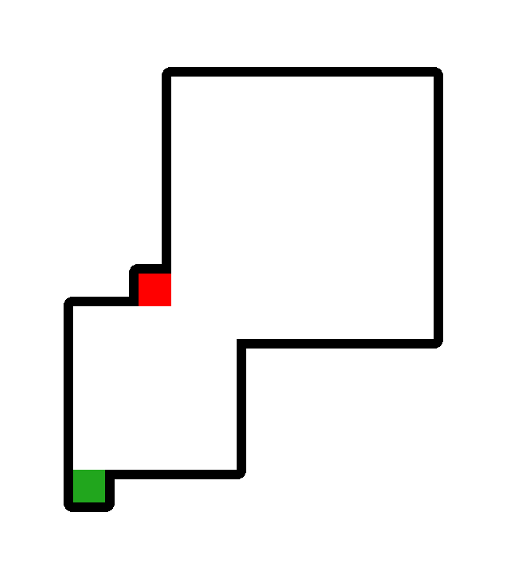
\includegraphics[width=\linewidth]{ab_divisive_2}
     		\caption{Map represented by $\langle 1,$\ $2, $\ $5  \rangle $\ $\langle4,$\ $6,$\ $8\rangle $\ $ \mid $\ $ \langle5,$\ $6,$\ $-10\rangle $\ $ \langle10,$\ $15,$\ $-6\rangle $\ $ \mid $\ $ \langle3, $\ $7, $\ $s\rangle $\ $ \langle1, $\ $1, $\ $d\rangle$.}
  	\end{subfigure}
  	\hfill
\caption{Two simple maps with their All-Black representation.}
\label{fig:allblack}
\end{figure}

% FRAMEWORK STRUCTURE % 

\section{Framework structure}

The framework collects data by assigning to the users \<matches> to play. A match is defined by the \<game mode> and by the \<map type>, which in turn is defined by the \<map topology> and by the \<map appearance>. The \<map topology> defines how the map is going to \<be> and depends on the algorithm used to generate it, whereas the \<map appearance> defines how the map is going to \<look> and depends on how the map is assembled. This implies that the map type defines a whole array of procedurally generated maps that share the same topology and appearance. Therefore, when referring to a match we are considering a specific game-mode played in a procedurally generated map. If needed, it is possible to use a pre-generated map instead of generating a new one, by providing it as input using one of the supported formats. In this case the \<map topology> defines how to interpret the input, that is then displayed considering the \<map appearance>.

\par

A match is defined by combining different modules, called \<Managers>, each of which controls a different aspect of the match.

% GAME MANAGER %

\subsection{The Game Manager}

The \<Game Manager> is the module responsible for the overall behavior of a match. Each game mode consists in a different version of the \<Game Manager>. It leans on the \<Map Manager> for the generation and the assembly of the map and on the \<Spawn Point Manager> for the spawn of entities. The \<Game Manager> controls the life-cycle of the match, that can be divided in the following phases:

\begin{itemize}
\item \<Setup>: all the modules are initialized.
\item \<Generation>: the \<Map Manager> generates or imports the map and assembles it.
\item \<Ready>: the \<Game Manager> displays a countdown announcing the start of the game.
\item \<Play>: the \<Game Manager> handles the game while the \<Experiment Manager> logs the actions of the player, if needed. This phase continues until an end condition is satisfied.
\item \<Score>: the \<Game Manager> stops the game and displays the final score.
\end{itemize}

% MAP MANAGER %

\subsection{The Map Manager}

The \<Map Manager> controls the generation, the import and the assembly of the map and the displacement of objects inside it. It leans on the \<Map Generator> for the generation, on the \<Map Assembler> for the \<assembly>\footnote{With \<assembly> we mean the operation of creating a 3D model of the map starting from its matrix representation.} and on the \<Object Displacer> for the \<displacement>\footnote{With \<displacement> we mean the operation of placing the 3D models of the objects in the assembled map, according to their position defined by the \<Map Generator> trough a \<positioning> algorithm.}, whereas it performs the import itself. If the map is provided in input as a text file, the \<Map Generator> is not called, whereas it is used to perform decoding if the map is provided in All-Black format.

\par

The framework provides three different versions of the \<Map Manager>.

\subsubsection{Single-Level Map Manager}

The \<Single-Level Map Manager> is used for any kind of single level map. It can generate maps, import them from file or decode them from All-Black format.

\subsubsection{Multi-Level Map Manager}

The \<Multi-Level Map Manager> is used for any kind of map that has more than one floor. It can generate multi-level maps or import them from file, but it cannot perform All-Black decoding. In addition to the standard modules, it employs a \<Stairs Generator> to position flight of stairs to connect the different floors. 

\par

Multi-level maps are obtained by using at least one generator to produce the desired number of floors. Since this allows to combine different kind of generators, we were able to obtain maps similar to the ones evolved by Cachia et al.\cite{MultiLevelEvolution} (see figure \ref{fig:multilevel_digger}), as well as maps with a more complex and interesting layout than the ones obtained by previous works (see figure \ref{fig:multilevel_divisive}).

\begin{figure}[tp]
	\centering
	\hfill
  	\begin{subfigure}[t]{0.45\linewidth}
	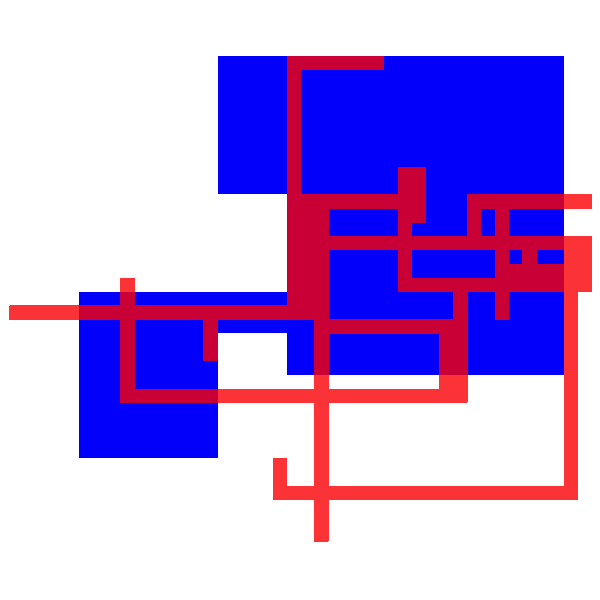
\includegraphics[width=\linewidth]{multilevel_digger}
	\caption{Multilevel map which floors have different topologies.}
	\label{fig:multilevel_digger}
 	\end{subfigure}
 	\hfill
  	\begin{subfigure}[t]{0.45\linewidth}
    			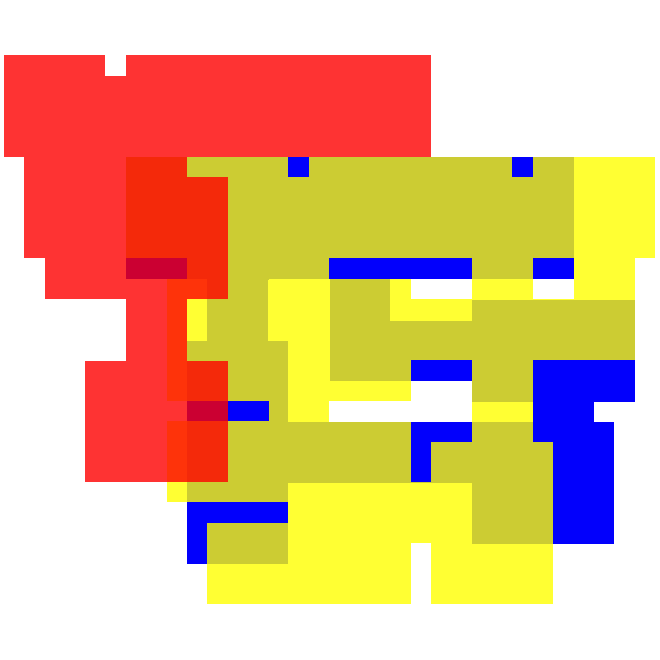
\includegraphics[width=\linewidth]{multilevel_divisive}
	\caption{Multilevel map which floors share the same topology.}
	\label{fig:multilevel_divisive}
  	\end{subfigure}
  	\hfill
\caption{Two multilevel maps.}
\end{figure}

\subsubsection{All-Black Multi-Level Map Manager}

The \<All-Black Multi-Level Map Manager> is used to decode multi-level maps saved in All-Black format. If no stairs are found among the objects, it employs the \<Stairs Generator> to position them.

% MAP GENERATOR %

\subsection{The Map Generator}

The \<Map Generator> controls the generation of the map. Each version of the \<Map Generator> defines a different \<map topology> depending on the used generation algorithm and on how its parametric settings are tuned. Some of these settings are shared by all the versions, whereas some of them are version-specific.

\par

The shared settings are used to define the size of the map and its encoding, to define the objects and to impose some constraints on their positioning:

\begin{itemize}
\item \<Width>: the number of rows of the matrix that represents the map.
\item \<Height>: the number of columns of the matrix that represents the map.
\item \<ObjectToObjectDistance>: the minimum number of cells that must separate two objects. 
\item \<ObjectToWallDistance>: the minimum number of cells that must separate an object and a wall.
\item \<BorderSize>: the width of the border placed all around the map once it has been generated, expressed in number of cells.
\item \<RoomChar>: the character used to represent a clear cell where the player can walk.
\item \<WallChar>: the character used to represent a filled cell where the player cannot walk.
\item \<MapObjects>: a list of the objects that must be placed in the map.
\end{itemize}

\noindent The objects contained in \<MapObjects> can represent spawn points, resources or decoration. They have the following properties:

\begin{itemize}
\item \<ObjectChar>: the character used to represent the object.
\item \<NumObjPerMap>: the number of objects of that kind that must be placed in the map.
\item \<PlaceAnywhere>: if this value is set to true, the restriction on the distance from the walls is ignored.
\item \<PositioningMode>: the algorithm used to position the object in the map.
\end{itemize}

\noindent The framework provides three different algorithms to position the objects inside the map:

\begin{itemize}
\item \<Rain>: positions the objects selecting random cells from the ones that are empty and satisfy the \<ObjectToWallDistance> constraint.
\item \<Rain Shared>: positions the objects selecting random cells from the ones that are empty and satisfy the \<ObjectToWallDistance> constraint and the \<ObjectToObjectDistance> constraint on the objects that have been placed using \<Rain Shared>.
\item \<Rain Distanced>: positions the objects selecting random cells from the ones that are empty and satisfy the \<ObjectToWallDistance> constraint and the \<ObjectToObjectDistance> constraint on the objects with the same \<ObjectChar>.
\end{itemize}

All of the following versions of the \<Map Generator> are deterministic, since they require a \<seed> value as input that constrains the output to a specific map.

% CELLULAR GENERATOR %

\subsubsection{Cellular Generator}

The \<Cellular Generator> employs a parametric \<cellular automaton>\footnote{A \<cellular automaton> consists of a grid of cells, each in one of a finite number of states, such as on and off. For each cell, a set of cells called its neighborhood is defined, usually composed by the ones that share at least one vertex with it (referred as \<8-neighbors>). Given the current state of the grid, a new generation is created, according to some fixed rule that determines the new state of each cell depending on the current state of the cell and of its neighbors.} to generate a natural looking map. 

\par

The algorithm starts by filling some tiles of the map selected at random, then it applies the cellular automaton for a certain number of generations and finally it performs some refinements (for more details, see algorithm \ref{alg:cellular}). The resulting topology depends on the following parameters:

\begin{itemize}
\item \<RandomFillPercent>: the percentage of tiles that are randomly filled during the initialization of the algorithm. High values promote narrow spaces, small values promote wide areas.
\item \<SmoothingInteration>: the number of generations the cellular automaton is ran for. High values penalize small features and make the walls smoother. 
\item \<NeighbourTileLimitLow>: the maximum number of neighbors a cell must have to became empty. Its value must be lesser or equal than the one of \<NeighbourTileLimitHigh>. The map becomes noisier the more they diverge.
\item \<NeighbourTileLimitHigh>: the minimum number of neighbors a cell must have to became filled.
\item \<WallThresholdSize>: the minimum number of cells that an isolated filled region must include to not be deleted. High values penalize small filled regions.
\item \<RoomThresholdSize>: the minimum number of cells that an isolated void region must include to not be deleted. High values penalize small empty regions.
\item \<PassageWidth>: the width of a passage connecting two different areas, expressed in number of cells.
\end{itemize}

\noindent Figure \ref{fig:cellulars} shows how these parameters influence the topology of a map.

\par

The \<Cellular Generator> can perform import and export using the text representation.

% DIVISIVE GENERATOR %

\subsubsection{Divisive Generator}\label{sssec:digger}

The \<Divisive Generator> employs a \<binary space partitioning algorithm> to generate a man-made looking map.

\par

The algorithm starts by obtaining partitions of the map by recursively dividing it in two sides of random size along one of the axes, then it selects some of these partitions as rooms and finally it connects them with corridors (for more details, see algorithm \ref{alg:divisive}). The resulting topology depends on the following parameters:

\begin{itemize}
\item \<RoomDivideProbability>: probability of a partition being divided again. High values promote small rooms.
\item \<MapRoomPercentage>: minimum percentage of tiles of the map that must be empty. High values promote close rooms separated by walls, low values promote distant rooms connected by corridors.
\item \<DivideLowerBound>: minimum division point expressed as percentage of the dimension of the room.
\item \<DivideUpperBound>: maximum division point expressed as percentage of the dimension of the room.
\item \<MinimumRoomDimension>: minimum width expressed in number of cells that a partition must have to be divided again. High values promote large rooms.
\item \<MinimumDepth>: the minimum number of recursive divisions that each partition must have experienced.
\item \<PassageWidth>: the width expressed in number of cells of the corridors connecting the rooms.
\item \<MaxRandomPassages>: the number of additional corridors to place, if possible, once that all the rooms are connected.
\end{itemize}

\noindent Figure \ref{fig:divisives} shows how these parameters influence the topology of a map.

\par

The \<Divisive Generator> can perform both import and export using the text representation, whereas the All-Black format is used only for export. The latter matches perfectly with this generator, since both are based on the concept of rooms and corridors.

% DIGGER GENERATOR &

\subsubsection{Digger Generator}

The \<Digger Generator> employs a simple algorithm to generate a man-made looking map.

\par

The algorithm is iterative and its state is defined by the current cell and by the current direction, that together with a randomly selected action determine the next cell that the algorithm is going to visit. Starting from the central cell of a filled map, at each iteration the algorithm empties the current cell and randomly decides if moving forward, turning left, turning right, jumping to a random visited cell or placing a flight of stairs, if controlled by a \<Multi-Level Generator>. The algorithm stops when a certain percentage of cells has been emptied. The resulting topology depends on the following parameters:

\begin{itemize}
\item \<ForwardProbability>: probability of moving forward in the next iteration. High values promote long corridors. 
\item \<LeftProbability>: probability of moving leftward in the next iteration. High values promote wide areas. 
\item \<RightProbability>: probability of moving rightward in the next iteration. High values promote wide areas. 
\item \<VisitedProbability>: probability of jumping to a visited cell in the next iteration. High values promote a more complex topology. 
\item \<StairProbability>: probability of placing a flight of stairs.
\item \<RoomPercentage>: percentage of tiles of the map that must be empty.
\end{itemize}

\noindent Figure \ref{fig:diggers} shows how these parameters influence the topology of a map.

\par

The \<Digger Generator> can perform both import and export using the text representation, whereas its own All-Black format is used only for import.

% GENERATORS ALGORITHMS AND IMAGES  %

\begin{algorithm}[tp]
\SetAlgoLined
\caption{Cellular generation algorithm.}
\algorithmfootnote{This algorithm is a modified version of the one proposed by Sebastian Lague\cite{lague}.}
\label{alg:cellular}

\For{every cell in the map}{
	empty the current cell\;
}

\While{percentage of filled cells $<$ RandomFillPercent} {
	select a random cell\;
	fill the selected cell\;
}

\For{generation from 0 to SmoothingIterations} {
	\For{every cell in the map}{
		count the 8-neighbors of the cell\;
		\If{8-neighbors  count $>$ NeighbourTileLimitLow}{
  			mark the current cell as filled for the next generation\;
   		}
		\If{8-neighbors  count $<$ NeighbourTileLimitHigh }{
  			mark the current cell as empty for the next generation\;
   		} 
	}
	update the map to the next generation\;
}

\For{every isolated region of empty cells}{
	\If{\#cells in the region $<$ RoomThresholdSize}{
		fill all the cells in the region\;
	}
}

\For{every isolated region of filled cells}{
	\If{\#cells in the region $<$ WallThresholdSize}{
		empty all the cells  in the region\;
	}
}

connect all the regions composed by empty cells\;
place the objects\;

\end{algorithm}

\begin{figure}[tp]
	\centering
  	\begin{subfigure}[t]{0.315\linewidth}
		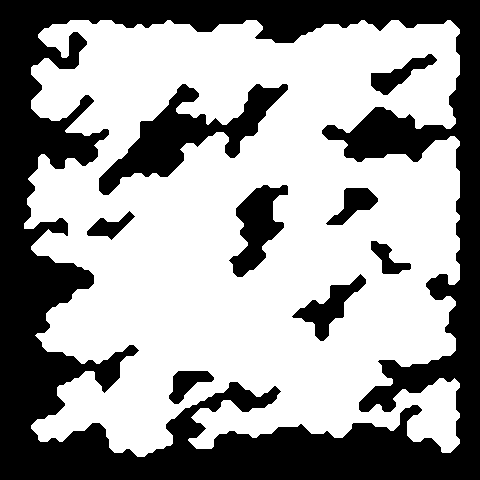
\includegraphics[width=\linewidth]{cellular_default}
     		\caption{Cellular map generated with the default settings.}
 	\end{subfigure}
 	\hfill
  	\begin{subfigure}[t]{0.315\linewidth}
    		
\includegraphics[width=\linewidth]{cellular_rfp40}
    		\caption{Cellular map generated with $Ran\-dom\-Fill\-Per\-cent = 40\%$.}
  	\end{subfigure}
  	\hfill
	\begin{subfigure}[t]{0.315\linewidth}
    		
\includegraphics[width=\linewidth]{cellular_rfp50}
    		\caption{Cellular map generated with $Ran\-dom\-Fill\-Per\-cent = 50\%$.}
  	\end{subfigure}
  	
  	\begin{subfigure}[t]{0.315\linewidth}
		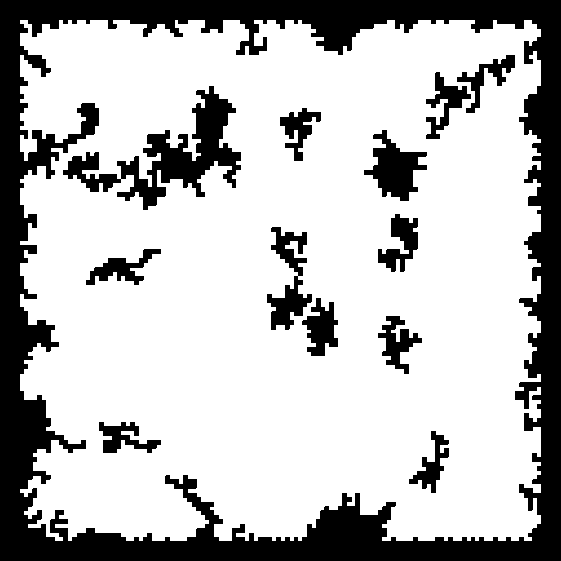
\includegraphics[width=\linewidth]{cellular_si0}
     		\caption{Cellular map generated with $Smooth\-ing\-It\-er\-a\-tions = 0$.}
 	\end{subfigure}
  	\hfill
  	\begin{subfigure}[t]{0.315\linewidth}
    		
\includegraphics[width=\linewidth]{cellular_si3}
     		\caption{Cellular map generated with $Smooth\-ing\-It\-er\-a\-tions = 3$.}
  	\end{subfigure}
  	\hfill
  	\begin{subfigure}[t]{0.315\linewidth}
    		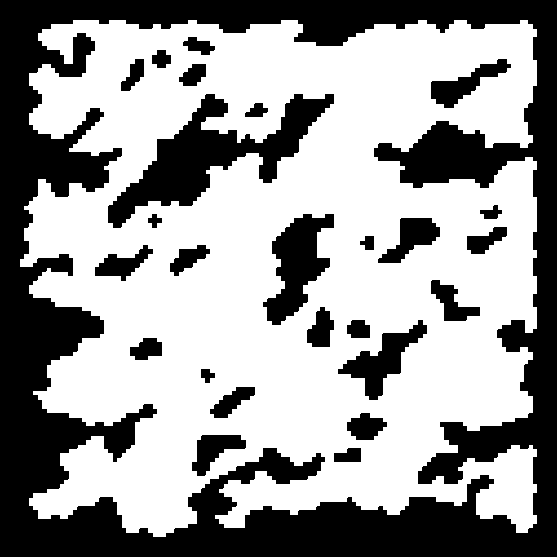
\includegraphics[width=\linewidth]{cellular_wts5}
     		\caption{Cellular map generated with $Wall\-Thresh\-old\-Size = 5$.}
  	\end{subfigure}	
	\caption[Six maps generated by the Cellular Generator using ``\<ANotSoRandomSeed>'' as seed, but different settings.]{Six maps generated by the Cellular Generator using ``\<ANotSoRandomSeed>'' as seed, but different settings. By default, the Cellular Generator has \<RandomFillPercent> set to $45\%$, \<SmoothingIterations> set to $2$,  \<NeighbourTileLimitHigh> set to $4$,  \<NeighbourTileLimitLow> set to $4$,  \<WallThresholdSize> set to $40$ and \<RoomThresholdSize> set to $100$.}
	\label{fig:cellulars}
\end{figure}

\begin{algorithm}[tp]
\SetAlgoLined
\caption{Divisive generation algorithm.}
\label{alg:divisive}

\For{every cell in the map}{
	fill the current cell\;
}

initialize the partitions list\;
DivideRoom(map, 0)\;

\While{percentage of empty tiles $<$ MapRoomPercentage}{
	extract a partition from the partitions list at random\;
	make the partition a room\;
	empty the tiles in the room\;
}

connect the rooms; 

\While{all the rooms are not directly connected \And \#placed additional corridors $<$ MaxRandomPassages}{
	add an additional corridor between two rooms selected at random;
}

place the objects\;

\hrulefill

\SetKwProg{Fn}{Function}{ is}{end}
\Fn{DivideRoom(section, depth)}{
	\eIf{(true with probability roomDivideProbability \And partition width $>$  minimumDividableRoomDimension \And partition heigth $>$ minimumDividableRoomDimension) \Or depth $<$  minimumDepth} {
		\eIf{previous division was horizontal} {
 			perform a random vertical division between \<divideLowerBound> and \<divideUpperBound>\;
		} {
 			perform a random horizontal division between \<divideLowerBound> and \<divideUpperBound>\;
		}
		DivdeRoom(first sub-section, depth + 1)\;
		DivdeRoom(second sub-section, depth + 1)\;
	}{
		add the partition to the partitions list;
	}	
}

\end{algorithm}

\begin{figure}[tp]
	\centering
  	\begin{subfigure}[t]{0.315\linewidth}
		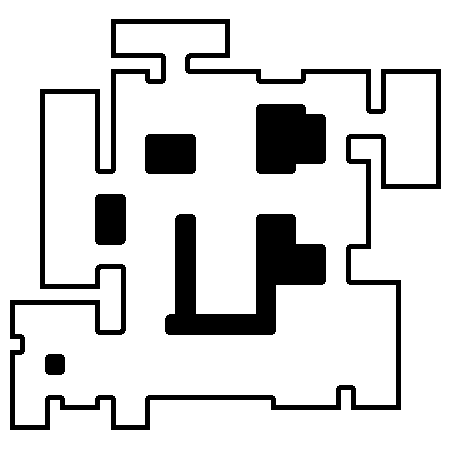
\includegraphics[width=\linewidth]{divisive_default}
     		\caption{Divisive map generated with the default settings.}
 	\end{subfigure}
	\hfill
  	\begin{subfigure}[t]{0.315\linewidth}
    		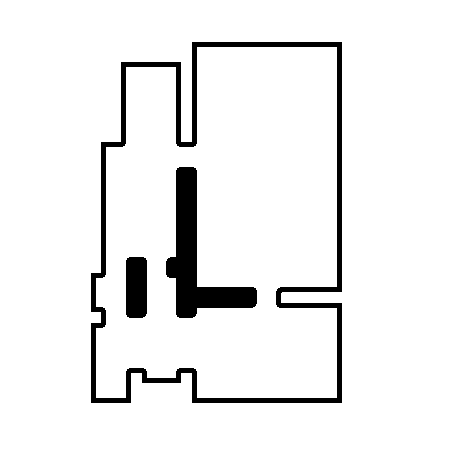
\includegraphics[width=\linewidth]{divisive_rdp20}
    		\caption{Divisive map generated with $Room\-Di\-vide\-Prob\-a\-bil\-i\-ty = 20\%$.}
  	\end{subfigure}
	\hfill
  	\begin{subfigure}[t]{0.315\linewidth}
    		
\includegraphics[width=\linewidth]{divisive_md1}
    		\caption{Divisive map generated with $Min\-i\-mum\-Depth = 1$.}
  	\end{subfigure}
  	
  	\begin{subfigure}[t]{0.315\linewidth}
		
\includegraphics[width=\linewidth]{divisive_md8}
     		\caption{Divisive map generated with $Min\-i\-mum\-Depth= 8$.}
 	\end{subfigure}
 	\hfill
  	\begin{subfigure}[t]{0.315\linewidth}
    		
\includegraphics[width=\linewidth]{divisive_mrd1}
     		\caption{Divisive map generated with $Min\-i\-mum\-Room\-Di\-men\-sion = 1$.}
  	\end{subfigure}
	\hfill
  	\begin{subfigure}[t]{0.315\linewidth}
    		
\includegraphics[width=\linewidth]{divisive_mrd7}
     		\caption{Divisive map generated with $Min\-i\-mum\-Room\-Di\-men\-sion = 7$.}
  	\end{subfigure}	
	\caption[Six maps generated by the Divisive Generator using ``\<AModeratelyRandomSeed>'' as seed, but different settings.]{Six maps generated by the Divisive Generator using ``\<AModeratelyRandomSeed>'' as seed, but different settings. By default, the Cellular Generator has \<Room\-Di\-vide\-Prob\-a\-bil\-i\-ty> set to $80\%$, \<Map\-Room\-Per\-cent\-age> set to $90\%$,  \<Di\-vide\-Low\-er\-Bound> set to $10\%$,  \<Di\-vide\-Up\-per\-Bound> set to $90\%$,  \<Min\-i\-mum\-Room\-Di\-men\-sion> set to $3$, \<Min\-i\-mum\-Depth> set to $4$, \<Pas\-sage\-Width> set to $3$ and \<Max\-Ran\-dom\-Pas\-sages> set to $12$.}
	\label{fig:divisives}
\end{figure}

\begin{figure}[tp]
\centering
\begin{subfigure}[t]{0.48\linewidth}

\includegraphics[width=\linewidth]{digger_default}
\caption{Digger map generated with the default settings.}
\end{subfigure}
\hfill
\begin{subfigure}[t]{0.48\linewidth}

\includegraphics[width=\linewidth]{digger_roomp20}
\caption{Digger map generated with $Room\-Per\-cent\-age = 20\%$.}
\end{subfigure}

\begin{subfigure}[t]{0.48\linewidth}

\includegraphics[width=\linewidth]{digger_fp60}
\caption{Digger map generated with $For\-ward\-Prob\-a\-bil\-i\-ty = 60\%$, $Right\-Prob\-a\-bil\-i\-ty = 19\%$ and $Left\-ward\-Prob\-a\-bil\-i\-ty = 19\%$.}
\end{subfigure}
\hfill
\begin{subfigure}[t]{0.48\linewidth}
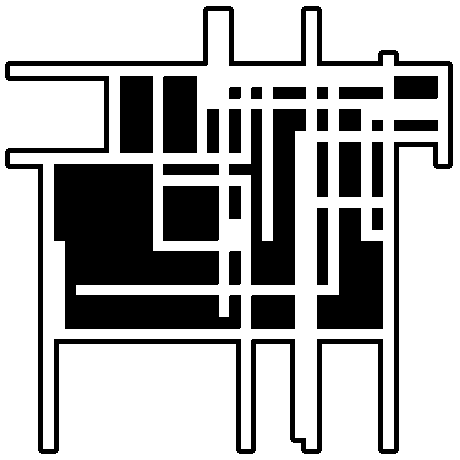
\includegraphics[width=\linewidth]{digger_fp96}
\caption{Digger map generated with $For\-ward\-Prob\-a\-bil\-i\-ty = 96\%$, $Right\-Prob\-a\-bil\-i\-ty = 1\%$ and $Left\-ward\-Prob\-a\-bil\-i\-ty = 1\%$.}
\end{subfigure}
\caption[Four maps generated by the Digger Generator using ``\<AFairlyRandomSeed>'' as seed, but different settings.]{Four maps generated by the Digger Generator using ``\<AFairlyRandomSeed>'' as seed, but different settings. By default, the Digger Generator has \<For\-ward\-Prob\-a\-bil\-i\-ty> set to $90\%$, \<Left\-Prob\-a\-bil\-i\-ty> set to $4\%$, \<Right\-Prob\-a\-bil\-i\-ty> set to $4\%$, \<Vis\-it\-ed\-Prob\-a\-bil\-i\-ty> set to $2\%$, \<Stair\-Prob\-a\-bil\-i\-ty> set to $0\%$ and \<Room\-Per\-cent\-age> set to $50\%$.}
\label{fig:diggers}
\end{figure}

% ALL-BLACK GENERATOR &

\subsubsection{All-Black Generator}

This simple generator parses inputs expressed in All-Black format, extracting rooms and corridors. If no objects are specified, it adds them to the map.

% STAIRS GENERATOR %

\subsection{The Stairs Generator}

The \<Stairs Generator> places stairs in the map after having analyzed it to find possible positions, but if stairs have already been placed by the \<Map Generator> (this happens with the \<Digger Generator>), it just validates them.

% MAP ASSEMBLER %

\subsection{The Map Assembler}

The \<Map Assembler> controls the assembly of the map. Each version of the Map Assembler corresponds to a different \<map appearance>.

% MESH ASSEMBLER %

\subsubsection{Mesh Assembler}

The \<Mesh Assembler> produces a 3D model of the map using an implementation of the \<marching squares algorithm>\footnote{\<Marching squares > is a computer graphics algorithm that generates contours for a \<two-dimensional scalar field>, i.e. a rectangular array of individual numerical values.} to generate three meshes: one for the floor, one for the walls and one for the ceiling. As it can be seen in figure \ref{fig:cellular_assembled}, the result is a natural-looking environment.

% PREFAB ASSEMBLER %

\subsubsection{Prefab Assembler}

The \<Prefab Assembler> produces a 3D model of the map by associating to each tile a specific 3D model, or \<prefab>, depending on the value of the tile and of its 8-neighbors (see figure \ref{fig:prefabs}). Figure \ref{fig:divisive_assembled} shows a map assembled with this algorithm.

\begin{figure}
\centering
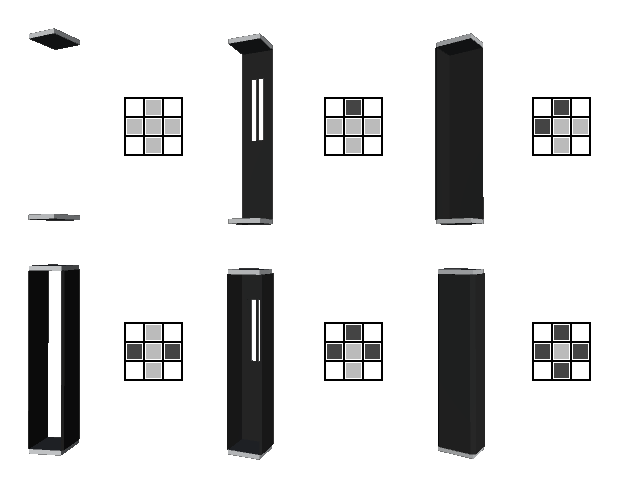
\includegraphics[width=0.95\linewidth]{prefabs}
\caption[Some prefabs and the masks they are associated to.]{Some prefabs and the masks they are associated to. Each model refers to the central cell of the corresponding mask. Green denotes empty cells, red denotes filled cell, half-green and half-red denotes cells that are ignored by the mask. The masks can be rotated to obtain all the possible configurations.}
\label{fig:prefabs}
\end{figure}

% MULTI-LEVEL PREFAB ASSEMBLER %

\subsubsection{Multi-Level Prefab Assembler}

Like the \<Prefab Assembler>, the \<Multi-Level Prefab Assembler> produces a 3D model of the map by combining prefabs, but it employs additional logic to manage the overlap of multiple floors. Figure \ref{fig:multi_assembled} shows a map assembled with this algorithm.

\begin{figure}
\centering
\begin{subfigure}[t]{0.48\linewidth}
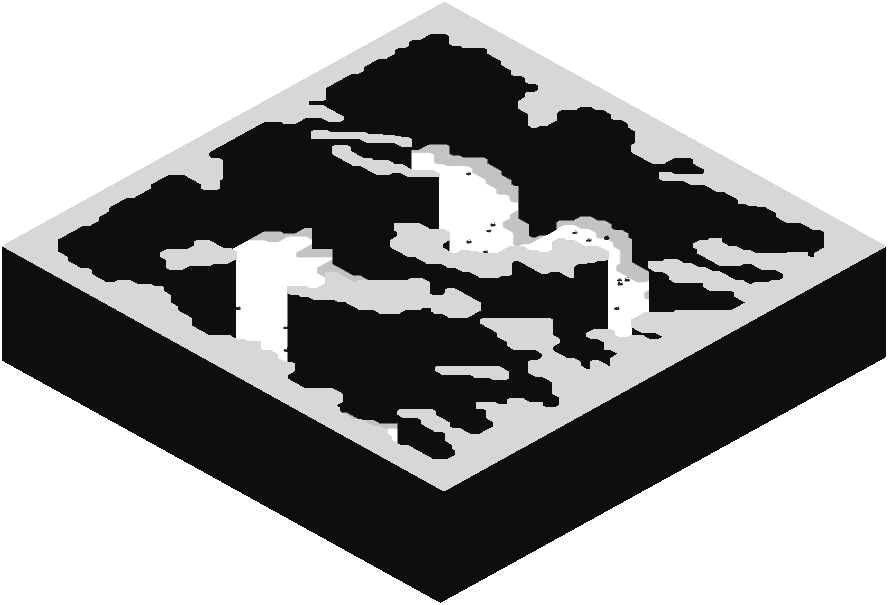
\includegraphics[width=\linewidth]{isometric_canyon}
\caption{Cellular map assembled with the \<Mesh Assembler>}
\label{fig:cellular_assembled}
\end{subfigure}
\hfill
\begin{subfigure}[t]{0.48\linewidth}
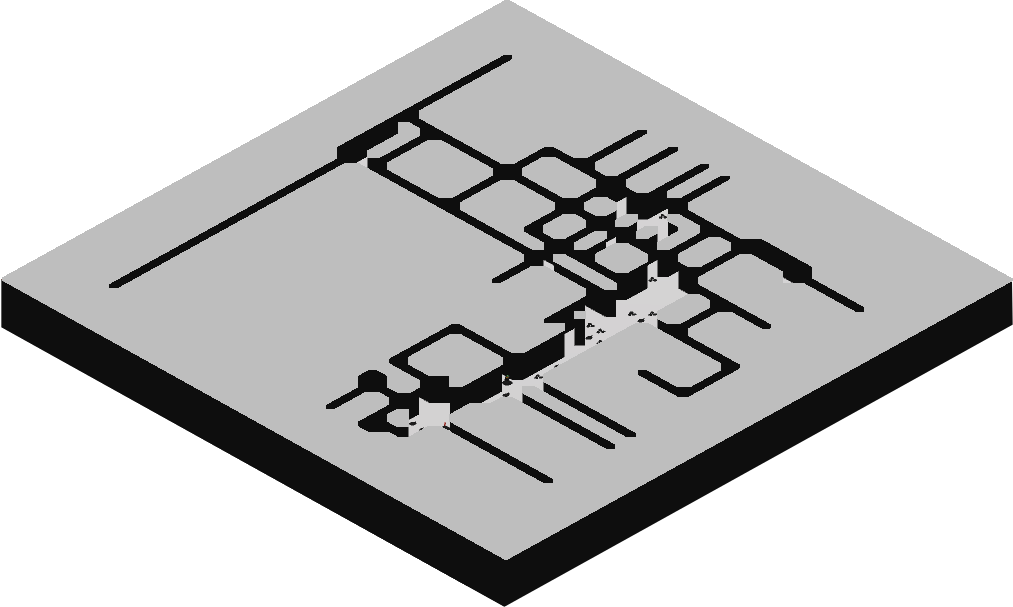
\includegraphics[width=\linewidth]{isometric_mine}
\caption{Digger map assembled with the \<Mesh Assembler>}
\label{fig:digger_assembled}
\end{subfigure}

\begin{subfigure}[t]{0.48\linewidth}
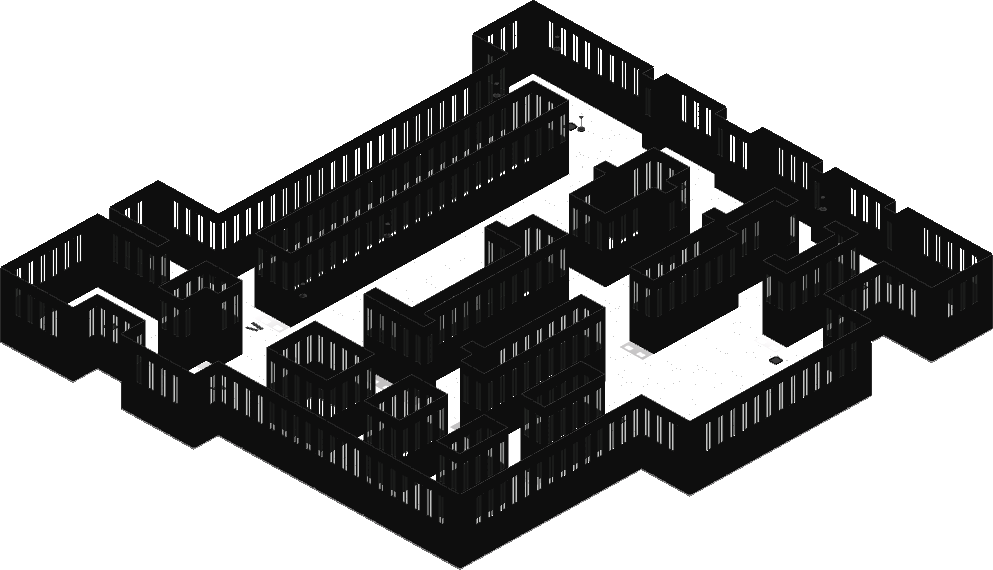
\includegraphics[width=\linewidth]{isometric_factory}
\caption{Divisive map assembled with the \<Prefab Assembler>}
\label{fig:divisive_assembled}
\end{subfigure}
\hfill
\begin{subfigure}[t]{0.48\linewidth}
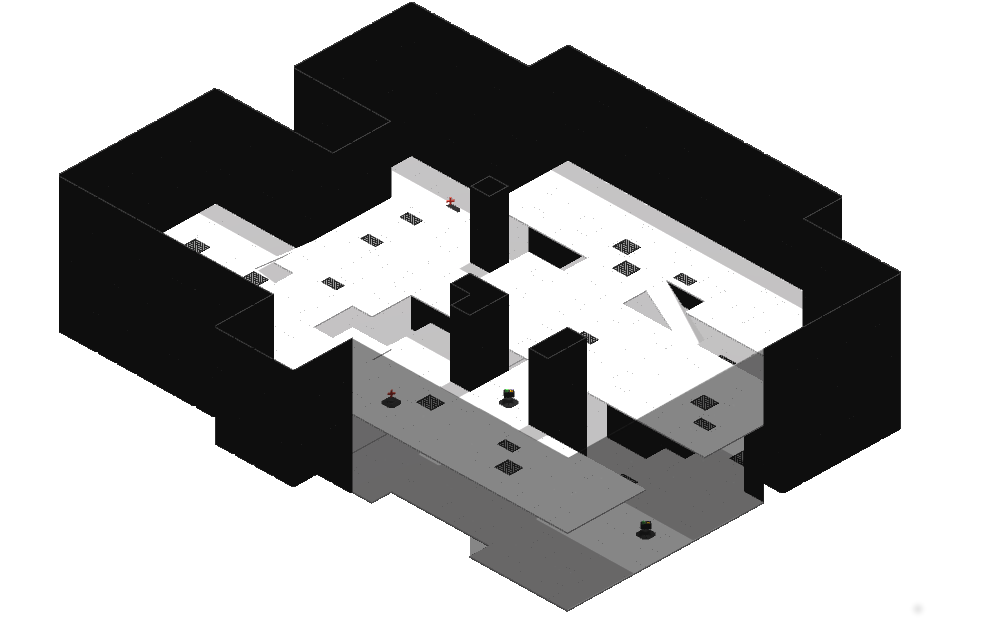
\includegraphics[width=\linewidth]{isometric_suburbs}
\caption{Multi-level map assembled with the \<Prefab Assembler>}
\label{fig:multi_assembled}
\end{subfigure}
\caption{Some possible combinations of generators and assemblers.}
\end{figure}

% SPAWN POINT MANAGER %

\subsection{The Spawn Point Manager}

The \<Spawn Point Manager> contains a list of all the spawn points displaced in the map, that is populated at the end of the \<Generation phase> by the \<Game Manager>. When the \<Game Manager> needs to spawn an entity, the \<Spawn Point Manager> provides a random spawn point from the ones that have not been used in a certain amount of time. If no spawn point meets this condition, the extraction is performed from the complete pool.

% OBJECT DISPLACER %

\subsection{The Object Displacer}

The \<Object Displacer> associates a character that represents neither a wall or a clear cell to the corresponding object, displacing it at the coordinates defined by its position in the map matrix. During this process, it populates a dictionary containing all the objects in the map divided by category, that is used by the \<Game Manager> to populate the list of spawn points used by the \<Spawn Point Manager>.

% EXPERIMENT MENAGER %

\subsection{The Experiment Manager}

The \<Experiment Manager> is a stand alone module that allows to create and manage the experiments used to perform user-based validation. Once that an experiment has been defined, the \<Experiment Manager> automatically assigns to the users the matches to play and collects the desired information.

\paragraph{Experiment definition}

\mbox{}\\

{\setlength{\parindent}{0cm}
An experiment is defined by a \<tutorial>, a list of \<studies> and a \<survey>.}

\par

The \<tutorial> is optional and consists in a match with a simple objective used to explain the commands to the user.

\par

The \<studies> are not optional and each one of them consists in a list of \<cases>. Each case contains a pool of maps and a single game mode, that is used to play the maps in the pool. The maps in the pool are the object of validation, whereas the game mode is the employed validation method.

\par

The \<survey> is optional and consists in a list of multiple-choice questions that are presented to the player at the end of the experiment.

\par

All these elements can be easily customized, as well as the number of test cases that an user has to play in a single experiment session, defined by the parameter \<CasesPerUsers>. The \<Experiment Manager> also allows to diagonally flip the maps, which is an useful method to avoid the rise of a bias due to memorization when the player is presented with different versions of the same map.

\paragraph{Experiment management}

\mbox{}\\

{\setlength{\parindent}{0cm}
Once that the experiment has been defined, it is ready to be played  by the users.}

\par

Each time that a user participates in the experiment, the \<Experiment Manager> selects the least played case of the least played study, in a round-robin fashion. This allows to have equally distributed data for each study and is possible thanks to the completion tracking provided by the \<Experiment Manager> itself. Then, for each case that the user is going to play, a pre-generated map is extracted from the pool and presented to the player as a match of the game mode specified by the case. In a complete experiment, the player will consecutively play the tutorial, one ore more matches and finally answer the survey.

\par

The experiment can be performed \<offline> or \<online>. In the former, the computed data and the experiment completion are stored locally, whereas in the latter, they are stored on a server. If the experiment is provided via an executable, then it is possible to configure it as \<offline>, \<online> or both, with the completion that is stored on a server and the computed data that is stored both locally and remotely. If the experiment is provided via a web build playable via browser, the only supported configuration is the \<online> one. 

\paragraph{Logging}

\mbox{}\\

{\setlength{\parindent}{0cm}
By default, the \<Experiment Manager> produces a complete log of each match, saving the following information:}

\begin{itemize}
\item \<MapInfo>: this field contains general information about the map featured in the match, as its name, its dimension, the size of its tiles and if it has been flipped.
\item \<GameInfo>: this field contains general information about the match, as the experiment name, the game mode and the duration.
\item \<SpawnLogs>: this field contains a list of all the spawn events. Each entry contains a timestamp, the coordinates of the spawn point and the name of the spawned entity.
\item \<PositionLogs>: this field contains a discretized list of the positions occupied by the player during the match, acquired with a given frequency. Each entry contains a timestamp, the coordinates of the player and the direction he is facing expressed in degrees.
\item \<ShotLogs>: this field contains a list of all the shots fired by the player. Each entry contains the same fields of the \<PositionLogs>, plus the identifier of the firing weapon, the number of projectiles in its magazine and its total available ammunition.
\item \<ReloadLogs>: this field contains a list of all the reloadings performed by the player. Each entry contains a timestamp, the identifier of the weapon that is being reloaded, the number of projectiles in its magazine and its total available ammunition, both before the reloading.
\item \<HitLogs>: this field contains a list of all the shots that hitted an entity. Each entry contains a timestamp, the coordinates of the hitted entity, the name of the hitted entity, the name of the hitter entity and the caused damage.
\item \<KillLogs>: this field contains a list of all the killings. Each entry contains a timestamp, the coordinates of the killed entity, the name of the killed entity and the name of the killer entity.
\end{itemize}

It is possible to customize the \<Experiment Manager> to have it compute and save specific metrics in a different log. Moreover, if the experiment includes a survey, the answers of the user are saved in a dedicated log.

\paragraph{Data retrieval}

\mbox{}\\

{\setlength{\parindent}{0cm}
The framework provides a simple interface for downloading the logs stored on the server. Since it is possible to set a limit on the dimension of logs which causes them to be split in multiple parts, the framework automatically performs merging and signals incomplete logs.
}

% ENTITIES %

\section{Entities}

The \<entities> are the \<agents> that take part in a match. All the entities share the following common features:

\begin{itemize}
\item \<TotalHealth>: the maximum number of health points of the entity, i.e. the quantity of damage the entity can receive before being destroyed.
\item \<Guns>: the guns associated to the entity.
\end{itemize}

The framework includes three different kind of agents:

\begin{itemize}
\item \<Player>: the entity that is controlled by the user. It can walk, jump, aim, deal and receive damage and pick resources.
\item \<Opponent>: this entity is similar to the one of the \<Player>, but in the current version of the framework it has no active logic, beside the one that controls its health.
\item \<Target>: this simple entity rotates in place. Besides receiving damage, it can harm the player thanks to the laser gun it can be equipped it. Figure \ref{fig:targets} shows different kind of targets.
\end{itemize}

\begin{figure}
\centering
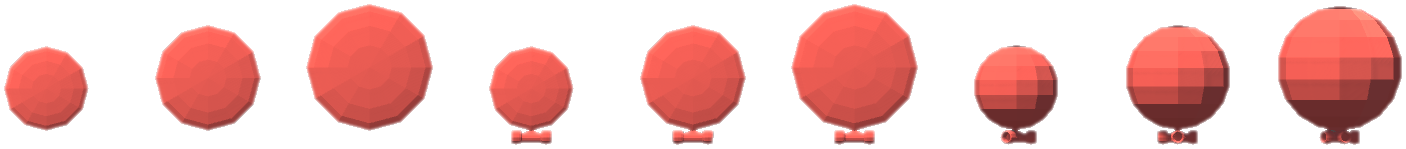
\includegraphics[width=0.95\linewidth]{targets}
\caption{Different ready-to-use target entities provided by the framework.}
\caption*{From the first to the third are simple targets, from the fourth to the sixth are targets equipped with two opposing laser guns, from the seventh to the ninth are``\<core>'' targets equipped with an increasing number of radial laser guns. The size of each target is proportional to its \<TotalHealth>.}
\label{fig:targets}
\end{figure}

% WEAPONS %

\section{Weapons}

The framework allows to easily define any kind of fire arm starting from a common parametric structure that characterizes the basic behavior of a gun with the following variables: 

\begin{itemize}
\item \<Damage>: the damage inflicted by a single projectile.
\item \<Dispersion>: the aperture of the cone-shaped projectile spread expressed in degree.
\item \<ProjectilePerShot>: the number of projectile emitted with one shot.
\item \<InfiniteAmmo>: tells if the gun has infinite ammunition.
\item \<ChargerSize>: the capacity of the gun magazine.
\item \<MaximumAmmo>: the maximum quantity of ammunition that can be carried for a specific gun.
\item \<ReloadTime>: the amount of time needed to reload the gun.
\item \<CooldownTime>:  the amount of time needed after a shot to fire again.
\item \<AimEnabled>: tells if the gun allows the player to aim.
\item \<Zoom>: the zoom provided by the scope when aiming.
\end{itemize}

\noindent This parametric approach allows to use the framework as a tool for user-based validation of procedurally generated weapons, that is another research field that has been explored in recent years \cite{ArmiProcedurali}.

\par 

The framework comes with three different categories of weapons already implemented.

\paragraph{Raycast guns}

\mbox{}\\

{\setlength{\parindent}{0cm}
\<Raycast guns> are weapons which projectiles have no \<time of flight>, but instantly hit the target once shot. The only additional parameter that this category introduces is \<Range>, which can be used to limit the reach of the weapon.
}

\par

There are three weapons of this category that the player can use:

\begin{itemize}
\item \<Assault Rifle>: a medium range weapon with a high fire rate, a capacious magazine and no dispersion which shots single medium damage projectiles. Figure \ref{fig:assault} shows its model and table \ref{tab:gunconfig} shows its parameters.
\item \<Shotgun>: a short range weapon with a slow fire rate, a small magazine and high dispersion which shots multiple low damage projectiles. Figure \ref{fig:shotgun} shows its model and table \ref{tab:gunconfig} shows its parameters.
\item \<Sniper Rifle>: a long range weapon with a slow fire rate, a small magazine and no dispersion which shots single high damage projectiles. It is equipped with a scope. Figure \ref{fig:sniper} shows its model and table \ref{tab:gunconfig} shows its parameters.
\end{itemize}

\paragraph{Projectile guns}

\mbox{}\\

{\setlength{\parindent}{0cm}
\<Projectile guns> are weapons that shoot projectiles with a limited flight speed. This category introduces two additional parameters:
}

\begin{itemize}
\item \<ProjectileLifetime>: if the projectile does not hit anything after this amount of time, it is destroyed.
\item \<ProjectileSpeed>: the speed of the projectile.
\end{itemize}

The only weapon of this category that the player can use is the \<Rocket Launcher>, a long range weapon with a slow fire rate, a small magazine and no dispersion which shots explosive projectiles. The projectiles of this weapon are slow and explode on impact, dealing an high damage that decreases radially from the center of the explosion. Figure \ref{fig:rocket} shows its model and table \ref{tab:gunconfig} shows its parameters.

\begin{figure}[p]
\centering
\begin{subfigure}[t]{0.48\linewidth}

\includegraphics[width=\linewidth]{gun_assault}
\caption{The Assault Rifle.}
\label{fig:assault}
\end{subfigure}
\begin{subfigure}[t]{0.48\linewidth}

\includegraphics[width=\linewidth]{gun_shotgun}
\caption{The Shotgun.}
\label{fig:shotgun}
\end{subfigure}
\begin{subfigure}[t]{0.48\linewidth}
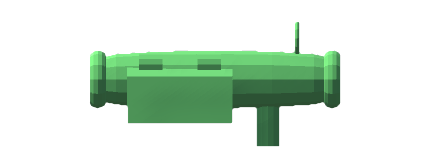
\includegraphics[width=\linewidth]{gun_rocket}
\caption{The Rocket Launcher.}
\label{fig:rocket}
\end{subfigure}
\begin{subfigure}[t]{0.48\linewidth}
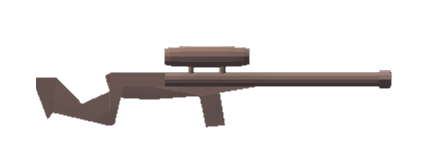
\includegraphics[width=\linewidth]{gun_sniper}
\caption{The Sniper Rifle.}
\label{fig:sniper}
\end{subfigure}
\caption{The weapons that the player can use.}
\end{figure}

\begin{table}[p]
\setlength\extrarowheight{2pt}
\begin{tabularx}{\textwidth}{|l|C|C|C|C|}
\cline{2-5}
\multicolumn{1}{c|}{}& Assault Rifle & Shotgun & Rocket Launcher & Sniper Rifle  \\
\hline
\<Damage> & 15  & 20  &  120 & 75  \\
\hline
\<Dispersion> & 0  & 7.5  & 0  & 0  \\
\hline
\<ProjectilesPerShot> &  1 &  5 & 1  & 1  \\
\hline
\<InfiniteAmmo> & false & false  & false &   false\\
\hline
\<ChargerSize> & 32  & 3  &  2 &  5 \\
\hline
\<MaximumAmmo> &  120 &  24 & 16  & 30  \\
\hline
\<ReloadTime> &  1 & 1  &  1 & 1  \\
\hline
\<CooldownTime> &  0.1 &  0.75 &  0.75 &  0.5 \\
\hline
\<AimEnabled> &  false & false  & false  & true  \\
\hline
\<Zoom> & 1  &  1 &  1 & 3  \\
\hline
\<LimitRange> & false  & true  &  - & false  \\
\hline
\<Range> &  - &  100 &  - &  - \\
\hline
\<ProjectileLifeTime> & -  & -  & 10  & -  \\
\hline
\<ProjectileSpeed> &  - &  - & 50 &  - \\
\hline
\end{tabularx}
\caption{Parametric configuration of the four weapons available to the player.}
    \label{tab:gunconfig}
\end{table}

\paragraph{Laser guns}

\mbox{}\\

{\setlength{\parindent}{0cm}
\<Laser guns> are not based on the same structure of the previous categories. Laser guns emit a continuous ray that deals damage over time to everything it touches. Their only configurable parameter is \<DPS> (\<damage per second>), i.e. the damage the the gun deals in a second when continuously hitting a target.
}

% OBJECTS %

\section{Objects}

Beyond \<decorations>, that are simple 3D models with no logic used to graphically enrich the map, the framework provides \<spawners>, i.e. objects that spawn a resource that can be collected by the entities. Once that the resource is collected, it disappears for an interval  of time defined by the parameter \<Cooldown>. The framework comes with two different \<spawners>:

\begin{itemize}
\item \<Health pack Spawner>: it spawns health packs, that partially restore the health of the entity. The healed amount of health is defined by \<RestoredHealth>.
\item \<Ammunition Spawner>: it spawns ammunition crates, that supply the entity with ammunition. \<SuppliedGuns> defines which guns the crates can supply, whereas \<AmmoAmounts> defines how many ammunition are provided to the entity for each supplied weapon.

\end{itemize}

% GAME MODES %

\section{Game modes}

The framework comes with three different game modes, that have been designed to highlight specific aspects of a multiplayer FPS. Each game mode is defined by a different version of the \<Game Manager>.

\subsection{Duel}

The \<Duel> game mode is a classic \<deathmatch> redistricted to two entities, with one of the two being the player. Each time that an entity eliminates the other one, it scores one point, whereas it loses one if it destroys itself by accident. When an entity has been eliminated, it \<respawns>\footnote{In video games, \<respawn> denotes the reappearing in a specific location, called \<spawn point>, of an entity which has been eliminated.} at a random spawn point. At the end of the match, which is marked by a time limit, the winner is the contender who has scored the highest number of points.

\par

Of the game modes that the framework provides, this one is the most complete, because it contains all the dynamics that characterize a multiplayer FPS match, and the most important, since it is the one that is usually used to perform validation in this research field.

\subsection{Target Rush}

\begin{figure}
\centering
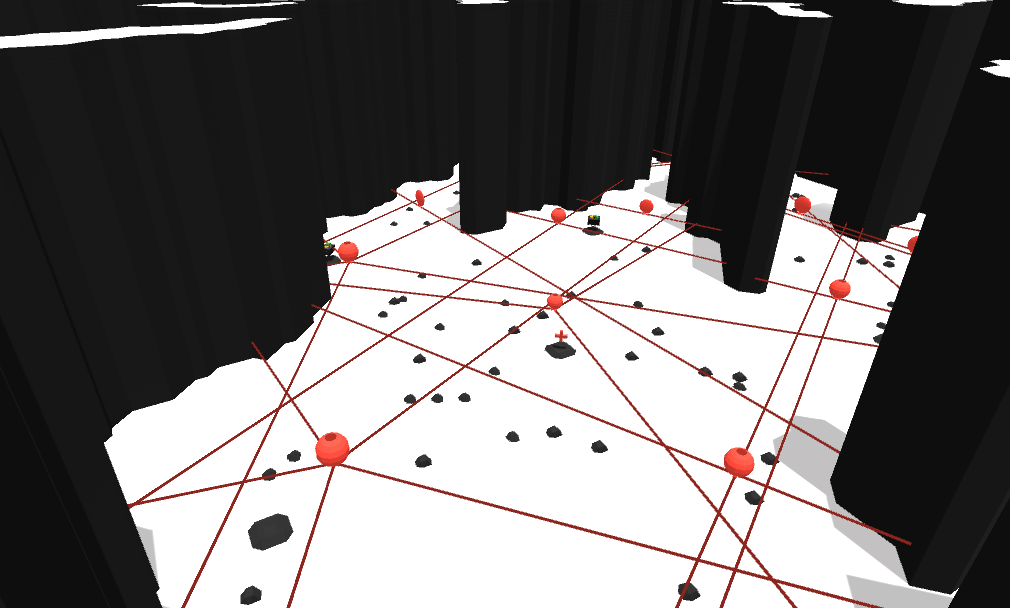
\includegraphics[width=0.95\linewidth]{rush20}
\caption{Targets equipped with laser guns in the final wave of a \<Target Rush> match.}
\label{fig:targets}
\end{figure}

In the \<Target Rush> game mode the player faces increasingly difficult waves of enemies, trying to obtain a score as high as possible before the end of the game, that is triggered by the player death or by the countdown hitting zero. The player earns points and additional time when he destroys an enemy or he completes a wave. The number of waves is parametric, as well as the content of each one. By default, this mode has twenty waves and uses targets as enemies, that start as harmless but became more and more numerous and dangerous with each wave (see figure \ref{fig:targets}). 

\par

This game mode has been designed to force the player to explore the map, through the research of enemies, health packs and ammunition, that quickly become indispensable as the match progresses.

\subsection{Target Hunt}

In the \<Target Hunt> game mode the player needs to find and eliminate a series of enemies in a given amount of time. The  enemies that the player is going to face are stored in a parametric list that is read circularly and are spawned one at a time, as soon as the previous one has been eliminated. To each enemy is assigned a score.

\par

This game mode has been designed to force the player to search a specific objective in the map.

\section{Summary}

In this chapter we analyzed the framework that we have developed to perform user-based validation, focusing on its structure, its components and its parametric nature.

% CHAPTER 4 - PYTHON FRAMEWORK %

\chapter{The graph-based tool}

% INTRODUCTION %

In this chapter we describe the tool that we have developed to perform analysis and populating of pre-generated maps using \<Graph Theory>. After a quick overview, we introduce the analysis capabilities of this tool and then we present how we have employed them, together with Graph Theory, to strategically place resources in pre-generated maps.

% DESCRIPTION %

\section{Description of the tool}

This tool generates different kind of graphs, starting from the text and the All-Black representation of a map, that are used to perform various analysis and manipulation operations.

\par

The use of All-Black format is convenient, because it provides by default a logical division of the map in different areas and it allows our tool to be applied by other researchers, since as we have seen the All-Black format is widely used in this field. We have used this tool to position resources in a pre-generated map, but, for instance, it could be used to address the identification and definition of design patterns from an unfamiliar perspective or for \<direct evaluation> in Search Based PCG.

\par 

We developed this tool in \<Python> because if offers many solid Graph Theory libraries, as \<NetworkX>, that is the one we have used.

% ANALYSIS %

\section{Analysis of pre-generated maps}

The analysis is performed by generating different kind of graphs, each one used to highlight a different feature of the map in question.

\subsection{Outlines graph}

The \<outlines graph> is generated starting from the All-Black representation of a map and is obtained by associating a node to every vertex of every room and corridor and by connecting the non-adjacent ones that belong of the same outline. This graph has a single kind of node (\<vertex node>), which contains the coordinates of the tile it represents, which are used to position the node when the graph is visualized. Figure \ref{img:graph_out} shows an example of this graph.

\par

This graph can be used to visualize the structures which compose the map.

\subsection{Reachability graphs}

Our tool can generate various kinds of \<reachability graphs> that represent various ways in which an entity can navigate a map. In these graphs a \<node> represents a position that an entity can reach, whereas an \<edge> indicates a viable path from a position to another.

\subsubsection{Tiles graph}

The \<tiles graph> is generated starting from the text representation of a map and is obtained by associating a node to each empty tile and by connecting each node to its corresponding 8-neighbors. The horizontal and vertical edges have cost $1$, whereas the diagonal ones have cost $\sqrt{2}$. This graph has a single kind of node (\<tile node>), which contains the coordinates of the tile it represents, which are used to position the node when the graph is visualized. Figure \ref{img:graph_tile} shows an example of this graph.

\par

This graph can be used to find the minimum distance that separates two cells, along with the shortest path that connects them.

\subsubsection{Rooms graph}

The \<rooms graph> is generated starting from the All-Black representation of a map and is obtained by associating a node to each room and corridor and by connecting nodes which corresponding rooms or corridors overlap with each other, using as weight the Euclidean distance of their central tile. This graph has a single kind of node (\<structure node>), used to represent both rooms and corridors, which contains the coordinates of the closest and furthest vertex of the structure from the origin. When visualized, each node is positioned on the coordinates of the central tile of the structure it represents. Figure \ref{img:graph_room} shows an example of this graph.

\par

This graph can be used to analyze the topology of a map, in order to find loops, choke points, central areas and other kind of structures.

\subsubsection{Rooms and resources graph}

The \<rooms and resources graph> is an extension of the room graph, which also include resources as nodes, that are connected to the nodes corresponding to the rooms and corridors which contain them. In addition to the structure node inherited form the rooms graph, this graph has a node to represent resources (\<resource node>), which contains the coordinates of the resource, which are used to visualize the node, and the character associated to the resource. Figure \ref{img:graph_room_res} shows an example of this graph.

\subsection{Visibility graph}

The \<visibility graph> is generated starting from the text representation of a map and is obtained by associating a node to each empty tile and by connecting each node to all the tiles that are visible from that node. For two tiles to be respectively visible, it must be possible to connect them with a line without crossing any filled tile. This graph has a single kind of node (\<visibility node>), which contains the coordinates of the tile it represents, which are used to position the node when the graph is visualized, and its \<degree centrality>, i.e. the number of edges incident to that node. 

\par

To make this graph easier to read by the user, the tool associates a color to the nodes, which ranges from blue, for the one with the minimum visibility, to red, for the one with the maximum visibility. This can be seen in figure \ref{img:graph_visibility}.

\par

This graph can be used to analyze which areas of the map are more exposed and which ones are more repaired.

\begin{figure}[]
	\centering
  	\begin{subfigure}[t]{0.45\linewidth}
		
\includegraphics[width=\linewidth]{graph_divisive}
     		\caption{The map.}
     		\label{img:graph_divisive}
 	\end{subfigure}
  	\begin{subfigure}[t]{0.45\linewidth}
    		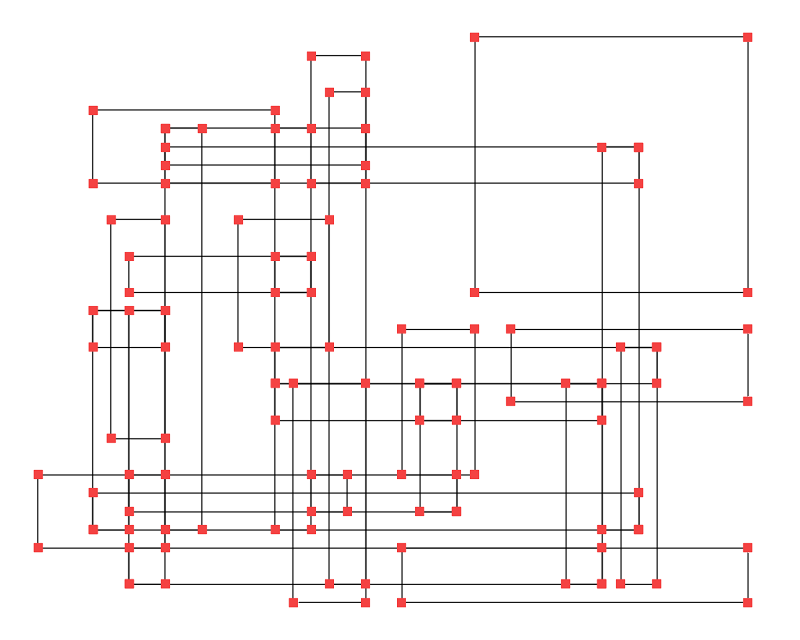
\includegraphics[width=\linewidth]{graph_out}
    		\caption{The outlines graph of the map.}
     		\label{img:graph_out}
  	\end{subfigure}
  	\begin{subfigure}[t]{0.45\linewidth}
    		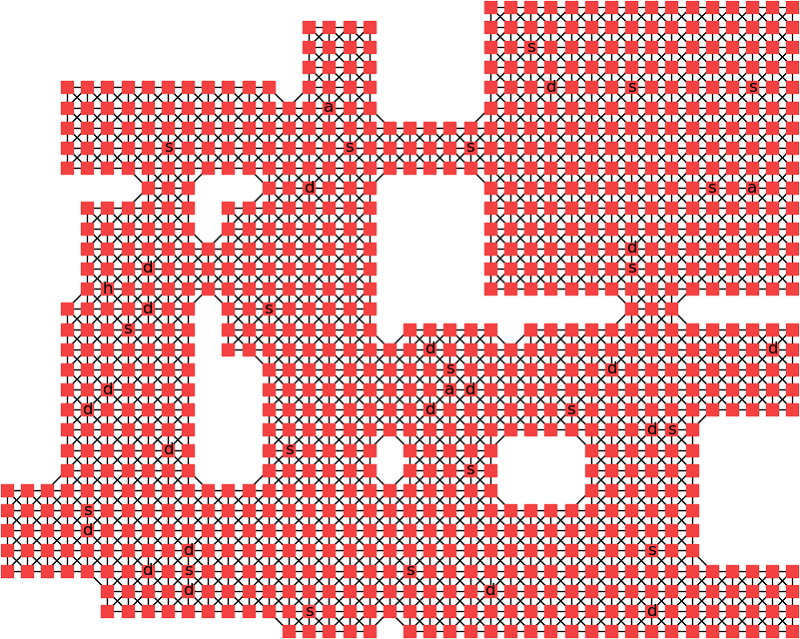
\includegraphics[width=\linewidth]{graph_tile}
    		\caption{The tiles graph of the map.}
     		\label{img:graph_tile}
  	\end{subfigure}
  	\begin{subfigure}[t]{0.45\linewidth}
    		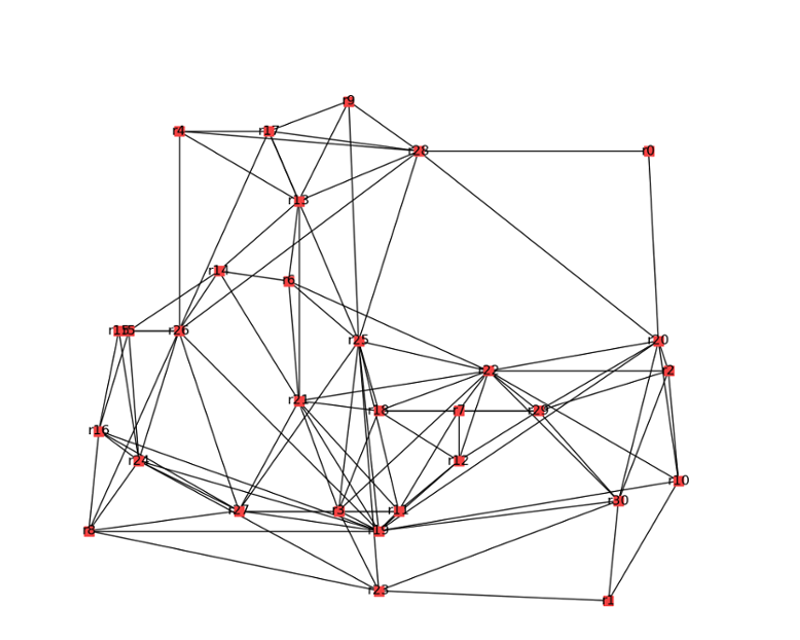
\includegraphics[width=\linewidth]{graph_room}
    		\caption{The rooms graph of the map.}
     		\label{img:graph_room}
 	\end{subfigure}
  	\begin{subfigure}[t]{0.45\linewidth}
    		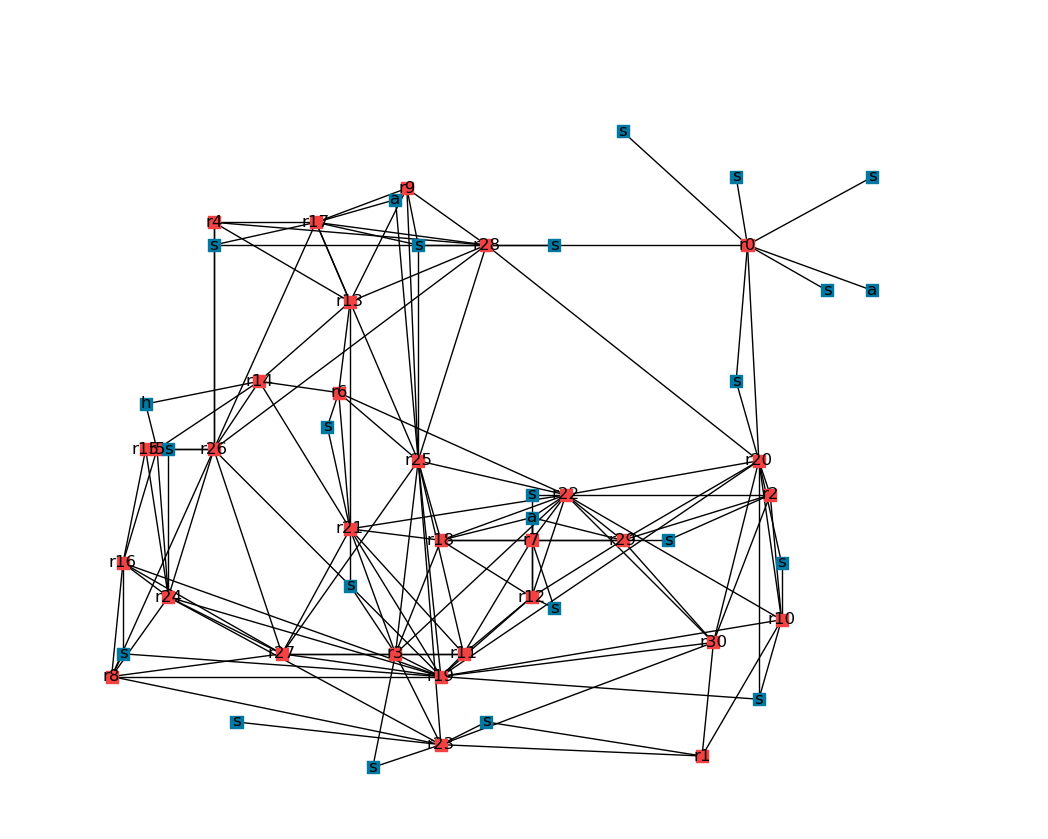
\includegraphics[width=\linewidth]{graph_room_res}
    		\caption{The rooms and resources graph of the map.}
     		\label{img:graph_room_res}
  	\end{subfigure}
  	\begin{subfigure}[t]{0.45\linewidth}
    		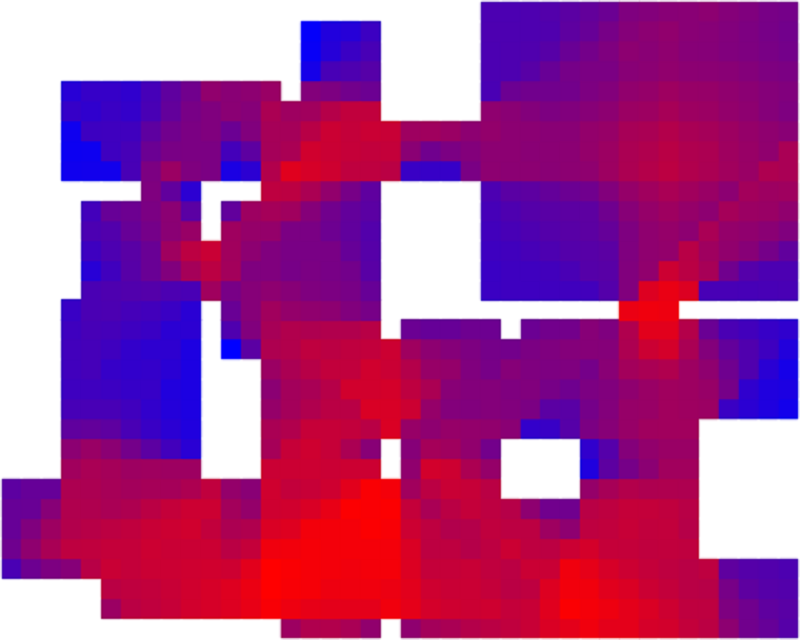
\includegraphics[width=\linewidth]{graph_visibility}
    		\caption{The visibility graph of the map.}
     		\label{img:graph_visibility}
  	\end{subfigure}	
	\caption{A map and all the graphs that the tool can generate from it.}
\end{figure}

\subsection{Interesting metrics}

Considering the graphs, in particular the ones with rooms and corridors as nodes, the following metrics defined by Graph Theory provide interesting information about the layout of a map:

\begin{itemize}
\item \<Degree centrality>: defined for a node, it is the number of edges that the node has. If the node represents a room, it measures how many entrance or exits the room has.
\item \<Normalized degree centrality>: defined for a node, it is obtained by normalizing the degree centrality, associating 0 to the node with the minimum centrality and 1 to the node with the maximum centrality.
\item \<Closeness centrality>: defined for a node, it measures its centrality in the graph, computed as the sum of the lengths of the shortest paths between the node and all other nodes in the graph. If the node represents a room, it measures how central the room is.
\item \<Betweenness centrality>: defined for a node, it measures its centrality in the graph, computed as the number of shortest paths connecting the nodes in the graph that pass through the node. If the node represents a room, it measures how central the room is.
\item \<Connectivity>: defined for a graph, it is the minimum number of elements (nodes or edges) that need to be removed to disconnect the remaining nodes from each other. If the graph represents a map, it measures the existence of isolated areas.
\item \<Eccentricity>: defined for a node, it is the maximum distance from the node to all other nodes in the graph. If the node represents a room, it measured how isolated the room is.
\item \<Diameter>: defined for a graph, it is the maximum eccentricity of its nodes. If the graph represents a map, it measures the size of the map.
\item \<Radius>: defined for a graph, it is the minimum eccentricity of its nodes. If the graph represents a map, it measures how distanced the rooms are from each other.
\item \<Periphery>: defined for a graph, it is the set of nodes with eccentricity equal to the diameter. If the graph represents a map, it defines its peripheral areas.
\item \<Center>: defined for a graph, it is the set of nodes with eccentricity equal to the radius. If the graph represents a map, it defines its central areas.
\item \<Density>: defined for a graph, it ranges from 0 to 1, going from a graph without edges to a complete graph. If the graph represents a map, it measures how complex it is.
\end{itemize}

% POPULATING %

\section{Populating of pre-generated maps}

We have defined multiple heuristics to populate a map with spawn points and resources using the metrics that can be extracted from a graph. These heuristic are a mathematical transposition of rules and patterns concerning resource placement that we have extracted from the work of Tim Schäfer\cite{great1vs1}, who has performed an in depth analysis of multiplayer 1vs1 maps for \<Quake 2>\footnote{Id Software, 1997}.


\subsection{FPS map analysis}

The balance of a deathmatch game radically changes each time that a player is killed. If the game has more than two players, the player who won the fight does not gain any strategic advantage, since he still has the other players to face, whereas the defeated player is put at considerable disadvantage, because on death he loses all the weapons and ammunition that he collected. In a 1vs1 match, a kill has an even stronger influence, since the surviving player has more weapons and ammunition and gains the complete control of the map, that comes with the chance of scoring another easy kill, as soon as the other player respawns, or of searching for additional equipment. Schäfer refers to the surviving player as \[up-player] and to the defeated one as \[down-player].

\par

To obtain a multiplayer map that is interesting and fun to play it is important to consider the up-player vs down-player dynamic both when defining the map layout and when positioning resources.

\par

The spawn points, i.e. the locations where the down-player reappears, should be positioned in areas that are of low interest for the up-player and that are easy to leave. Obviously, central hubs and dead ends are a bad choice, whereas rooms with 2 or 3 exits are usually the best option. 

\par

For what concerns the resources, they must be placed considering both the up-player vs down-player dynamic and the characteristics of the resource itself. It is important to place the right amount of resources on the map, because too many would eliminate the need for exploration, whereas too few would further disadvantage the down player. It is also important not to place too many powerful items in the same area or in boring spots, since the risk to obtain them should always be proportional to the strategical advantage they allow to achieve. It is important to consider that a powerful resource is interesting for both players, so it often acts as a \<point of collision>. The resources usually are of five kinds: health pack, armor, power-up, ammunition and weapon. 

\par

The health packs are placed in zones that are safe or not too dangerous. They have no use for the down-player, that respawns with full health, but they can be useful for the up-player, if he has been damaged during the fight, whereas they always come in handy during a fight or when one of the contenders disengages.

\par

Armor, which is a second health that is consumed before the main one, is usually placed in spots that are aimed both at the down-player and at the up-player: objects that provide a small quantity of armor should be easy to achieve, whereas the ones that provide full armor should be placed in dangerous areas.

\par

Power-ups grant temporary advantages to the player who collects them, like invisibility or increased damage, and are placed in locations difficult to reach. 

\par 

The position of a weapon and of its ammunition depends on the weapon itself. We can divide the weapons in three categories: weak, medium and strong. Weak weapons are of a certain interest for the down-player, if he has not collected any other weapon yet, and of no interest for the up-player, so they are placed near spawn-points or in gaps where no other weapon is available, together with their ammunition. Medium weapons are of high interest for the down-player, since he needs to get one of them as soon as possible if he wants to face the up-player, so they are placed in areas that are easy to reach and the same goes for their ammunition. Finally, the strong weapons should be placed in areas that are strategically disadvantageous, like dead ends or vertically dominated areas, or difficult to reach. If a weapon is very contextual, i.e. it is useful in very few situations, it is usually placed in an area that allows to take advantage of its features, whereas a weapon that is strong in almost any situation is usually placed in an area where it cannot be used optimally (e.g. a rocket launcher in a small room).

\subsection{Spawn points placement}

We have defined four heuristics for the placement of spawn points. 

\subsubsection{Low risk heuristic}

We defined an heuristic that places spawn points in the rooms that have the minimum number of entrances but are not dead ends and are distant enough from each other. Inside the room, the spawn point is placed on the tile that has the lowest visibility but is not adjacent to the wall. In this way spawn points are placed in passageways that are sheltered and easy to leave. At each iteration, we select a structure from the \<rooms and resources graph> using the following heuristic, given $G$ the rooms and corridors graph, $S \subset G$ the subset of structure nodes, $R \subset G$ the subset of resource nodes and $n$ the number of spawn points that must be added to the map:

\begin{align*}
room = \argmin_{s \in S} & \vast\{ w_1 \times
	\begin{cases}
    		\hfil 1 & \text{if } \degcent(s) = 1 \\
    		\cfrac{\degcent(s) - \min_{s' \in S}\degcent(s')}{\max_{s' \in S}\degcent(s') - \min_{s' \in S}\degcent(s')} & \text{if } \degcent(s) \neq 1 \
  	\end{cases} \vast\} \\ 
  	 &\quad +  w_2 \times \min_{n \in G}
  	\begin{cases}
    		\hfil 1 & \text{if } n \in S \\
    		\cfrac{\spl(r, n)}{\diam(G)} & \text{if } n \in R \
  	\end{cases} \vast\} \\ 
  	 &\quad +  w_3 \times \cfrac{| r \in R \, / \, r \in \neigh(s) |}{n}	
	\vast\}
\end{align*}

The first component of the equation, which is weighted by $w_1$, penalizes rooms depending on the number of passages they have, the second component, which is weighted by $w_1$, penalizes rooms close to a spawn point, and the third component, which is weighted by $w_3$, penalizes rooms that already contain one or more spawn points. All the three components are normalized in the interval $[0,1]$ so that their influence on the final result is proportional to their weight. We experimentally found that the values that provide the best results are:

$ w_1 = 1 , w_2 = 0.5,  w_3 = - 2$

\subsubsection{High risk heuristic}

\subsubsection{Uniform heuristic}

\subsubsection{Random heuristic}

\subsection{Ammunition placement}

\subsection{Health packs placement}

% SUMMARY %

\section{Summary}

% CHAPTER 5 - FIRST EXPERIMENT %

\chapter{Experiment on spawn points placement heuristics}

% INTRODUCTION %

In this chapter we describe the experiment that we have performed for validating the placement heuristics for spawn points described in the previous chapter and, at the same time, for testing the data-collection capabilities of our framework, that was used to setup and manage the experiment.

% DESCRIPTION %

\section{Description}

With this experiment we analyzed how the placement of spawn points influences the up-player vs down-player dynamic. The experiment tries to recreate the situation where the up-player, once killed his opponent, tries to find him as soon as possible, just after his respawn, to score another easy kill. As we have seen, a well-designed map should slow down this operation by having its spawn points in areas that are not central, are easy to leave and covered. The \<low risk> heuristic described in chapter \ref{sss:lowrisk} has been designed to place the spawn points according to such criteria, so, to prove its effectiveness, we decided to confront how this facet of the up-player vs down-player dynamic changes with respect to spawn points placed with the \<uniform> heuristic, defined as well in chapter \ref{sss:uniform}, which selects the areas to contain spawn to be distributed evenly inside the map.

\par

To highlight this particular dynamic, we designed a game mode where the user, which represents the up-player, must find and destroy a static target, which represents the down-player, as many times as possible before times runs out. Each time that the user destroys a target, it respawns at a random spawn point. The user cannot die and has infinite ammunition, so he does not have to look for resources.

% SETUP %

\section{Setup}

For this experiment, we setup the \<Experiment Manager> to propose in each play session a quick tutorial, two matches and a survey. The experiment was composed by three \<studies>, corresponding to different pre-generated maps, each one composed by two \<cases>, one that corresponded to the \<low risk> spawn points distribution and one that corresponded to a pool of five \<uniform> spawn point distributions. In a play session, the user played the same map twice, once with the low risk distribution and once with one of the uniform distributions, in a random order and with the map flipped in one of the two matches. We used the survey to profile how much the user was familiar with video games and FPS, to evaluate his skill and to get a feedback about in which of the two maps it was harder to find the targets. The experiment was deployed online and played by the users via browser on their own computer.

\par

Each match had \<Target Hunt> as game mode. The duration of the match was set to three minutes, the list of spawnable entities consisted of just one target and the only weapon available to the player was the \<assault rifle> with infinite ammunition. The pre-generated maps were stored as text files and were loaded by the \<Divisive Generator> and displayed with the \<Prefab Assembler>. 

\par
 
For each match, a complete game log was saved, along with the following performance metrics, saved in a separate log:
 
 \begin{itemize}
\item \<TargetLogs>: this field contains a list of all the targets that the user managed to destroyed. Each entry contains a timestamp of when the target was destroyed, the coordinates of the target, the coordinates of the user, the distance covered by the user and the time passed during the lifespan of the target.
\item \<Shots>: the total number of projectiles shot by the user.
\item \<Hits>: the number of projectiles that hit a target.
\item \<Accuracy>: the percentage of projectiles that hit a target.
\item \<Kills>: the total number of targets destroyed by the user.
\item \<Distance>: the total distance covered by the user during the match, considering cells of unitary width.
\item \<AvgKillTime>: the duration of the match divided by the number of kills.
\item \<AvgKillDistance>: the total distance divided by the number of kills.
\end{itemize}

\noindent
The answers to the survey were saved as well.
 
 \par
 
The performance of the player is measured by \<AvgKillTime>, that is also an indicator of how difficult it is to find targets in the map.

\par
  
We have selected three procedurally generated maps that present radically different layouts and we populated each one of them using both the low risk and the uniform heuristic:

\begin{itemize}
\item \<Arena>: this map presents a wide open arena, two sides of which are adjacent to parallel corridors with many openings. As the visibility heatmap in figure \ref{img:arena_visibility} shows, the central arena allows to control most of the map, whereas the corridors offer some repair and perfect spots to place spawn points. Figure \ref{img:arena_safe} shows the spawn points positioned using the low risk heuristic, whereas figure \ref{img:arena_uniform} shows one of the five configuration produced using the uniform heuristic.
\item \<Corridors>: this map presents many small rooms connected by long corridors. As it can be seen in figure \ref{img:corridors_visibility}, there is no area that allows to control the others and the only point with high visibility are the ones where corridors intersect. Figure \ref{img:corridors_safe} shows the spawn points positioned using the low risk heuristic, whereas figure \ref{img:corridors_uniform} shows one of the five configuration produced using the uniform heuristic.
\item \<Intense>: compared to the previous two, this map presents an intermediate layout, since it has both open areas and small rooms connected by corridors. As it can be seen in figure \ref{img:intense_visibility}, this reflects also on the visibility, that is high in the central open arenas and low in the remaining sections of the map. Figure \ref{img:intense_safe} shows the spawn points positioned using the low risk heuristic, whereas figure \ref{img:intense_uniform} shows one of the five configuration produced using the uniform heuristic.
\end{itemize}

\par

It is important to observe that the low risk and the uniform heuristics select rooms to place a spawn point with two different criteria, but they employ the same logic when selecting a tile inside a room. This means that the two heuristics select tiles which have similar visibility conditions, so the player's performance difference depends exclusively on how the rooms have been selected. This is observable in figures \ref{img:arena}, \ref{img:corridors} and \ref{img:intense}: when the uniform heuristics happens to select a room that has been selected also by the low risk one, the spawn point is placed exactly on the same tile.

\begin{figure}[tp]
	\centering
	\begin{subfigure}[t]{0.3\linewidth}
    		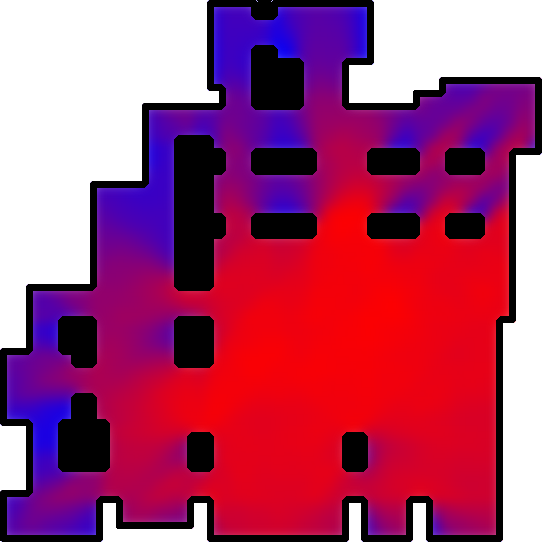
\includegraphics[width=\linewidth]{arena_visibility}
     		\caption{Heatmap showing the visibility of the level.}
		\label{img:arena_visibility}
  	\end{subfigure}  	
  	\hfil
  	\begin{subfigure}[t]{0.3\linewidth}
    		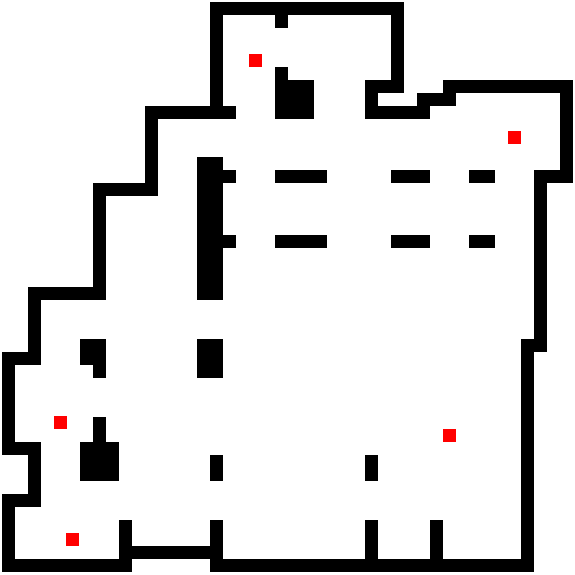
\includegraphics[width=\linewidth]{arena_safe}
     		\caption{Spawn points (in red) placed using the safe heuristic.}
     		\label{img:arena_safe}
  	\end{subfigure}
  	\hfil
  	\begin{subfigure}[t]{0.3\linewidth}
    		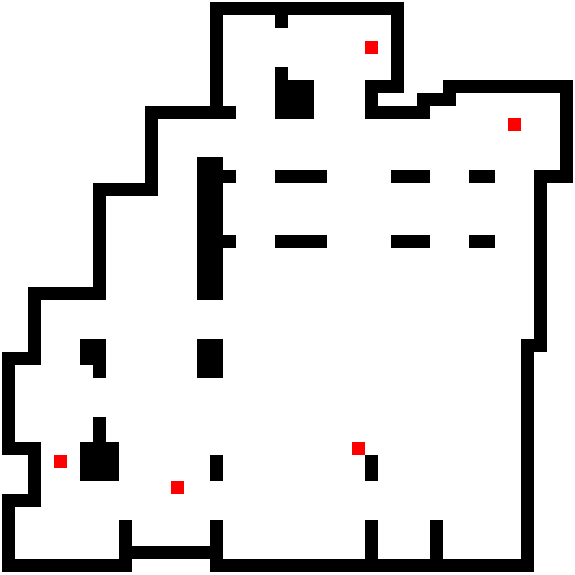
\includegraphics[width=\linewidth]{arena_uniform}
     		\caption{Spawn points (in red) placed using the uniform heuristic.}
		\label{img:arena_uniform}
  	\end{subfigure}  
	\caption{``Arena'' map used in the experiment.}
	\label{img:arena}
\end{figure}

\begin{figure}[tp]
	\centering
  	\begin{subfigure}[t]{0.3\linewidth}
    		
\includegraphics[width=\linewidth]{corridors_visibility}
     		\caption{Heatmap showing the visibility of the level.}
		\label{img:corridors_visibility}
  	\end{subfigure}  	  
  	\hfil
  	\begin{subfigure}[t]{0.3\linewidth}
    		
\includegraphics[width=\linewidth]{corridors_safe}
     		\caption{Spawn points (in red) placed using the safe heuristic.}
     		\label{img:corridors_safe}
  	\end{subfigure}
  	\hfil
  	\begin{subfigure}[t]{0.3\linewidth}
    		
\includegraphics[width=\linewidth]{corridors_uniform}
     		\caption{Spawn points (in red) placed using the uniform heuristic.}
		\label{img:corridors_uniform}
  	\end{subfigure}	
	\caption{``Corridors'' map used in the experiment.}
	\label{img:corridors}
\end{figure}

\begin{figure}[tp]
	\centering  	
  	\begin{subfigure}[t]{0.3\linewidth}
    		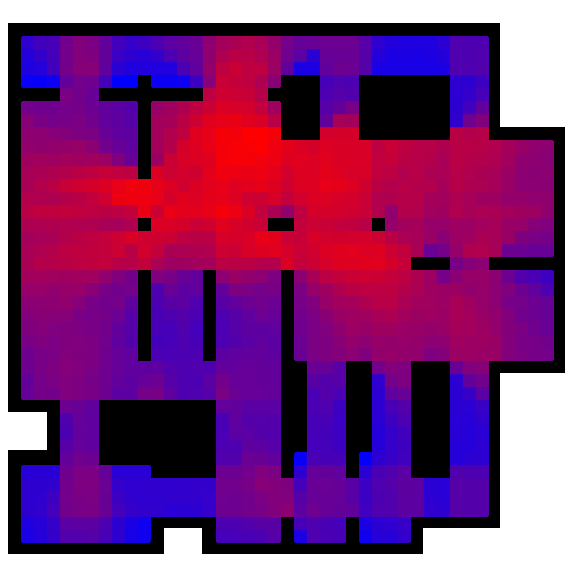
\includegraphics[width=\linewidth]{intense_visibility}
     		\caption{Heatmap showing the visibility of the level.}
		\label{img:intense_visibility}
  	\end{subfigure}  	
  	\hfil
  	\begin{subfigure}[t]{0.3\linewidth}
    		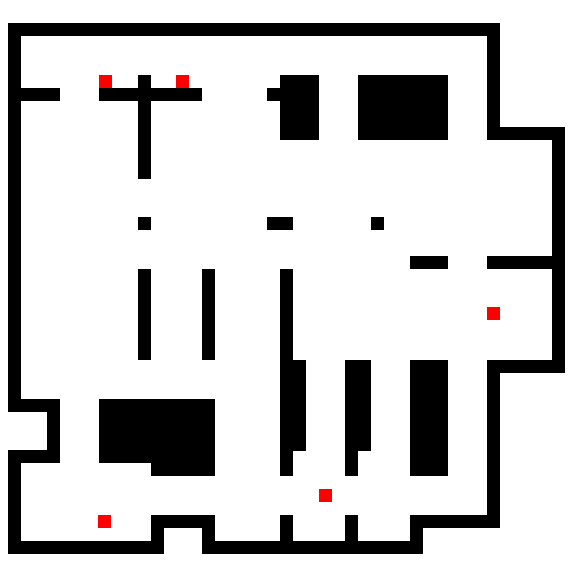
\includegraphics[width=\linewidth]{intense_safe}
     		\caption{Spawn points (in red) placed using the safe heuristic.}
     		\label{img:intense_safe}
  	\end{subfigure}
  	\hfil
  	\begin{subfigure}[t]{0.3\linewidth}
    		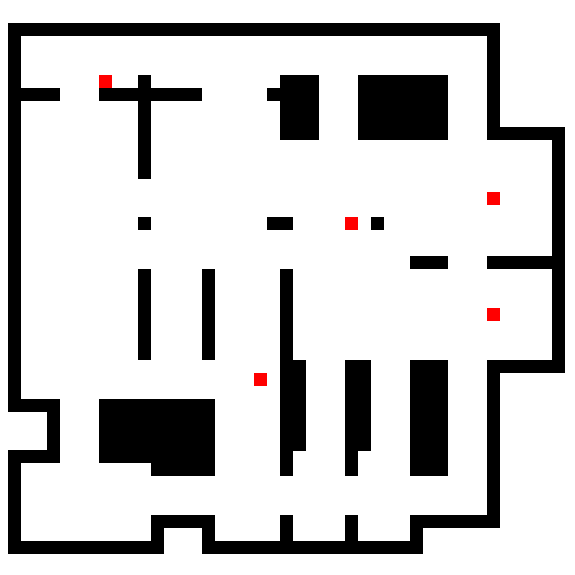
\includegraphics[width=\linewidth]{intense_uniform}
     		\caption{Spawn points (in red) placed using the uniform heuristic.}
		\label{img:intense_uniform}
  	\end{subfigure}
	\caption{``Intense'' map used in the experiment.}
	\label{img:intense}	
\end{figure}

% RESULTS %

\section{Results}

\begin{figure}[tp]
	\centering  	
  	\begin{subfigure}[t]{0.48\linewidth}
    		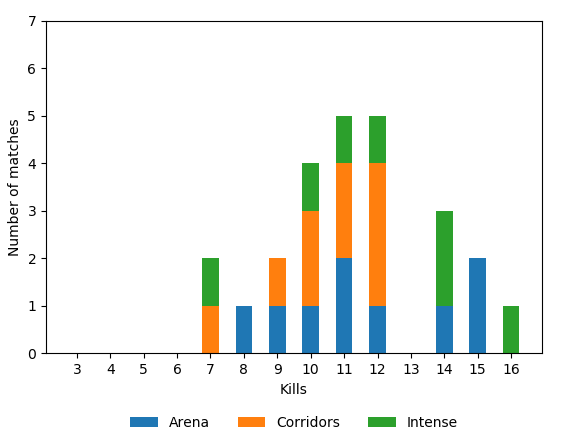
\includegraphics[width=\linewidth]{bar_lowrisk}
     		\caption{Low risk heuristic.}
		\label{img:bar_lowrisk}
  	\end{subfigure}  	
  	\hfil
  	\begin{subfigure}[t]{0.48\linewidth}
    		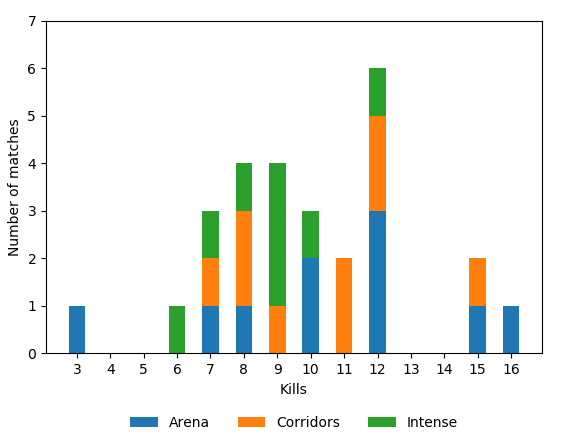
\includegraphics[width=\linewidth]{bar_uniform}
     		\caption{Uniform heuristic.}
     		\label{img:bar_uniform}
  	\end{subfigure}
	\caption[Distribution of the matches by number of kills for the two heuristics.]{Distribution of the matches by number of kills for the two heuristics. The matches are also classified by map.}
	\label{img:intense}	
\end{figure}

% CONCLUSIONS %

\section{Conclusions}



% CHAPTER 6 - SECOND EXPERIMENT %

\chapter{Conclusions}

% CONCLUSIONS %

The purpose of this thesis was to create a framework to perform research in procedural content generation for First Person Shooters. Past works have employed open source games, like Cube 2, that allow to perform validation via artificial agents but present many limitations when it is needed to collect information from real users. There was therefore the need of a way to collect data online, in an easy and quick way, and we answered to it by designing our framework to deploy browser playable experiments, that once defined collect data automatically.

\par

Being aimed at research, we wanted our framework to be as versatile as possible, so we opted for a modular and parametric design that is easy to customize and we included many generation algorithms and map representation formats that have been used in previous works. We included the All Black format, defined by Cardamone et al.\cite{Cardamone:2011:EIM:2008402.2008411}, that is a standard in the literature, but we extended it to be more complete and flexible, introducing variable genome size, game elements codification and multi-level support. Because we expect multi-level generation to be a topic of great interest in the years to come, we included the multi-level map format defined by Cachia et al.\cite{MultiLevelEvolution}, who were the first to evolve multi-level maps, but we also extended the classic All-Black representation to be multi-level. This, together with the possibility of including the position of game elements and stairs, should allow to perform evolution of multi-level maps starting from what has already been done in single level research. 

\par

Moreover, we explored how Graph Theory can be applied to level design, with regard to both map analysis and placement of game elements, and we found various graphs and metrics that allow to extract interesting information from a map starting from its All-Black representation. Then, we designed an approach that allows to employ this information to place game element in a meaningful way, considering the different requirements of each object, that we defined by analyzing how level design influences the up-player vs down-player dynamic.

\par

Finally, we tested our framework by performing an experiment to analyze how the placement of spawn points influences the up-player vs down-player dynamic. With this experiment we were able to validate the placement methods that we have defined and we managed to observe how the map layout influences the disposition of game elements. In this way, we proved our graph-based approach to be useful both for map analysis and for the contextual positioning of game elements.

% ISSUES %

\section{Known issues and possible criticism}

The main issue with the framework is that it does not have neither artificial agents nor the support for online multiplayer and this limits its possible applications.

\par

For what concerns graph analysis, the rules that we have defined for placing game elements could be criticized for a lack of a strong theoretical basis, since as we have seen there is still no common ground for what concerns level design. Moreover, we assigned the weights used in the placement heuristics empirically, making various attempts and choosing the weights that produced the disposition of game elements most coherent with the rules we defined. Despite this, the experiment proved both the rules and the weight assignment to be effective.

% FUTURE %

\section{Future developments}

Two major features that should be implemented in the framework are an artificial intelligence for agents and the support for online multiplayer, since they would allow to significantly increase the possible applications of our work. Moreover, to make the framework more complete and allow to directly generate well designed maps, it would be a great improvement to implement the map analysis and the game element placement directly in the framework, instead of performing them using an external tool. Unlucky, we were forced to keep them separated since \<C\#>, that we used to develop the framework, does not have any solid graph library.

\par

In chapter \ref{ss:interesting_metrics} we listed many metrics that can give interesting information about the layout of a map, but we have used only some of them to define the placement heuristics. An interesting development would be to include more of them, in particular the ones that allow to define areas of the map, like \<Periphery> and \<Center>. As we have highlighted, weapons require a specific treatment when positioned, since their overall damage, strengths and weakness should influence their place in the map, and such metrics can be employed to define the areas that better suit each weapon. Another improvement would be the extension of the analysis performed via graph to multi-level maps. Moreover, as we have already highlighted in the thesis, the graphs we have defined could be used for the individuation and analysis of design patterns.

\par

Finally, it would be interesting to design an evolutionary process that generates maps and places resources using a fitness function addressed to the up-player vs down-player dynamic.

% CHAPTER 7 - CONCLUSIONS %

\include{chapters/chapter7}

% BACK MATTER %

\backmatter

% BIBLIOGRAPHY %

\bibliography{bibliography} 
\bibliographystyle{ieeetr}

\end{document}